% =====================================================================
% body.tex -- the ENTIRE paper, shared verbatim by both wrappers
% (single_column.tex, two_column.tex). No \documentclass here, no
% variant-conditional text. Wide floats use the widefigure/widetable
% environments defined in preamble_shared.tex (figure*/table*).
% =====================================================================

\title{Geometry-Aware Neural Operator Surrogates for External Aerodynamics:
       Physics Consistency, Out-of-Distribution Generalization
       and Calibrated Uncertainty}

\author{T.~Amin}
\email{taimooramin419@gmail.com}
\noaffiliation

\date{\today}

\begin{abstract}
Geometry-conditioned neural surrogates are reported as accurate on external
aerodynamics benchmarks, but almost always in one narrow sense: field or drag
error, in distribution, with no check on whether a prediction is internally
consistent or the reported uncertainty means anything. We audit three
geometry-conditioning families (a $k$-nearest-neighbour graph network, a
signed-distance-conditioned Fourier neural operator in the GINO style, and a
Transolver-style geometry transformer), each reimplemented at matched parameter
count ($\sim$1.3--1.4\,M) and training budget, under a single protocol built
around force self-consistency, generalization across six evaluation splits,
and calibrated uncertainty. The central instrument is force self-consistency
(\FSC): the disagreement between the drag obtained by quadrature of a model's
own predicted surface pressure and the drag from a regression head on the same
backbone. \FSC{} needs no ground truth, so it is computable out of distribution
and on unlabelled candidate geometries. On AirfRANS, with the force integrator
gated against the dataset's own coefficients (median relative error
$3.3\times10^{-4}$), three findings recur across all three architectures. Field
accuracy separates the models cleanly (transformer $>$ operator $>$ graph net,
everywhere, by up to $4\times$), but $C_D$ rank correlation from the coefficient
head does not: all three sit at $\rho_s\approx0.94$--$0.999$, and a 29-parameter
ridge baseline reaches $0.83$--$0.90$ on every split. Ranking drag by
integrating the predicted fields is weaker still, no better than ridge for the
best model and far worse for the graph net, so the two drags a single model
reports disagree by 5--24\% in distribution and up to 115\% under shift, which
is exactly what makes \FSC{} a working label-free shift detector. Split
conformal prediction holds near nominal coverage in distribution for two of the
three models but its guarantee does not survive flow-regime shift, and an
uncertainty-driven acquisition score, verified against independent Ansys Fluent
RANS runs, concentrates its picks in the corner of the design space where the
steady solver itself struggles; on the two post-stall cases the solver could
settle, the surrogates were off by $640$--$900\times$ their in-distribution
error. Code, split manifests, and the Fluent verification set are released.
\end{abstract}

\maketitle
\raggedbottom

% =====================================================================
\section{Introduction}
\label{sec:intro}
% =====================================================================

The external-aerodynamics surrogate literature has converged on a narrow
scoreboard: relative $L_2$ error on velocity and pressure fields, plus an error
or rank correlation on drag. Papers get accepted on that scoreboard. Engineers
cannot use it, for three reasons.

\textbf{Gap 1: internal inconsistency is invisible.} Models are trained with a
field loss and, sometimes, a separate head for integrated coefficients. Nothing
forces the predicted surface pressure and wall shear stress to integrate to the
predicted drag. A model can be accurate in field norm while being internally
inconsistent about the one number (an integrated force coefficient) a designer
actually acts on, because force is a small difference of large, partially
cancelling contributions dominated by regions (leading-edge suction peak,
separation onset, base pressure) that carry little weight in a domain-averaged
norm. That internal gap is a cheap, ground-truth-free diagnostic almost nobody
reports; we make it a first-class measurement, and it turns out to be large:
tens of percent of the true drag, growing with shift
(\S\ref{sec:results_consistency}).

\textbf{Gap 2: out-of-distribution failure is acknowledged but not
characterized.} Reported gains are almost always measured on random,
in-distribution splits, while deployment means new operating points and new
shapes. Prior benchmarking work states plainly that OOD generalization remains
a challenge for every method tested \citep{rabeh2025benchmarking}, which is a
conclusion, not a characterization. Which axis of shift hurts most: Reynolds
number, angle of attack, or shape family? We evaluate on six splits spanning
four shift axes (data scarcity, Reynolds number, angle of attack, shape
family) plus a fifth split that shifts shape and Reynolds together, the hardest
cell, and report every metric against split identity rather than as a single
aggregate (\S\ref{sec:protocol}).

\textbf{Gap 3: uncertainty is reported without calibration.} Where uncertainty
is reported at all it is usually an ensemble spread: a heuristic score, least
trustworthy under exactly the shift where it matters, rarely checked against
realised coverage and almost never checked \emph{under shift}. Split conformal
prediction converts any such score into finite-sample coverage under
exchangeability, a genuine guarantee in distribution and a measurable failure
mode out of it, yet conformal coverage for aerodynamic surface fields and
derived coefficients has not been systematically reported.

\paragraph{Contributions.}
\begin{enumerate}\itemsep2pt
  \item \textbf{C1: force self-consistency (\FSC)} as a label-free diagnostic,
        defined in \S\ref{sec:protocol} and evaluated on every split.
  \item \textbf{C2: a matched-budget audit} of three geometry-encoding families
        (graph, SDF-conditioned FNO, geometry transformer) under one protocol,
        one data pipeline and one training budget, including data-efficiency
        curves and targeted ablations.
  \item \textbf{C3: calibration under shift}: deep ensembles plus split
        conformal prediction, with coverage, interval width and ECE reported
        per split and the exchangeability assumption stated where it breaks.
  \item \textbf{C4: a solver-verified loop}, in which an acquisition score
        built from ensemble spread and \FSC{} selects candidate cases that are
        then run in Ansys Fluent, a solver independent of the one that
        generated the training data, with a grid-independence study and a
        measured solver offset so the comparison is interpretable.
\end{enumerate}

\begin{widefigure}
  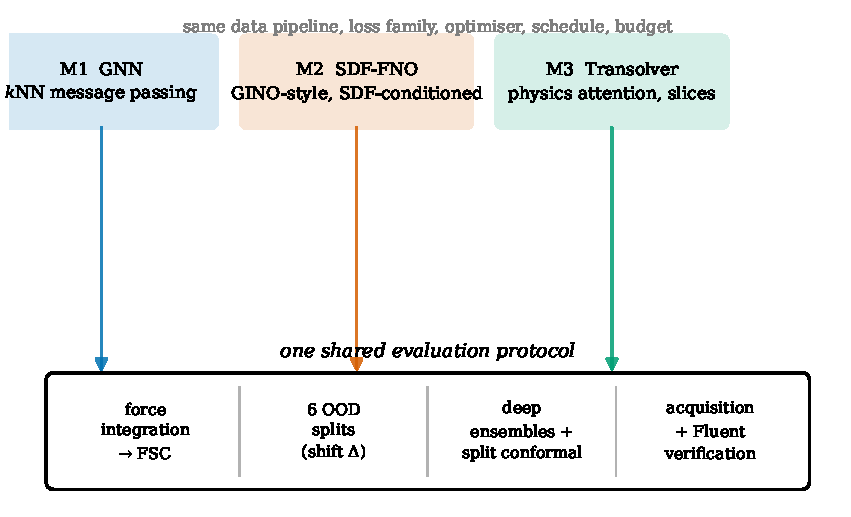
\includegraphics[width=\figwidthfull]{figures/fig01_schematic.pdf}
  \caption{The three geometry-encoding families and the shared evaluation
           protocol beneath them: only the encoder changes; the force
           integration, the six OOD splits, the ensembling/conformal
           calibration and the acquisition/Fluent loop are identical across
           \Mgnn, \Mfno{} and \Mtrans.}
  \label{fig:schematic}
\end{widefigure}

% =====================================================================
\section{Related work}
\label{sec:related}
% =====================================================================

\paragraph{Neural operators and geometry encoding.}
Fourier neural operators \citep{li2021fno}, their geometry-informed extension
\citep{li2023gino}, and the general operator-learning framework
\citep{kovachki2023neuraloperator} together with DeepONet \citep{lu2021deeponet}
and mesh-based graph networks \citep{pfaff2021meshgraphnets} define the design
space. Transolver \citep{wu2024transolver} represents the attention-based branch.

\paragraph{Benchmarks for flow around complex geometry.}
AirfRANS \citep{bonnet2022airfrans} supplies the dataset, the metric definitions
and the Reynolds and angle-of-attack splits this study inherits.
\citet{rabeh2025benchmarking} is the closest prior art and the framing anchor: it
compares operators and foundation models across geometry encodings. Our axis is
consistency and calibration rather than an accuracy ranking, so we cite it as
motivation rather than as a competitor. DrivAerNet++ \citep{elrefaie2024drivaernetpp}
provides the 3D extension. \citet{takamoto2022pdebench} and
\citet{ohana2024thewell} set the benchmark-documentation conventions we follow.

\paragraph{Physics-consistency losses.}
Physics-informed operators \citep{li2021pino} penalise PDE residuals during
training. We use the same machinery diagnostically: residuals are reported
whether or not they are penalised, which is what separates a measurement from
a training trick.

\paragraph{Uncertainty quantification.}
Deep ensembles \citep{lakshminarayanan2017ensembles} for the predictive spread;
split conformal prediction \citep{angelopoulos2021gentle, vovk2005algorithmic,
lei2018distributionfree} for distribution-free intervals, with
\citet{romano2019cqr} as an alternative score. \citet{tibshirani2019covariateshift}
is why our shape-family results are framed as a documented failure of
exchangeability rather than as a bug.
\citet{vinuesa2022enhancing} frames the CFD-community reception.

% =====================================================================
\section{Problem setup and the consistency protocol}
\label{sec:protocol}
% =====================================================================

This section is the conceptual core of the paper: the shared operator-learning
formulation, the force-integration route to a coefficient, the consistency
diagnostic built from the gap between that route and a learned head, and the
shift axes along which every model is evaluated.

\subsection{Operator learning setup}
Let $\dom \subset \R^d$ be the fluid domain exterior to a body with boundary
$\bnd$, and let $\cond$ be the flow condition; for the airfoil case
$\cond = (\Uinf, \aoa)$ with $\Rey = \Uinf \chord / \nu$. We seek
\begin{equation}
  \Sop : (\geom, \cond) \longmapsto u = (\bv, p, \nut)\big|_{\dom},
\end{equation}
restricted in practice to the surface trace
$\Sbnd : (\geom,\cond) \mapsto (\cp, \tauw)\big|_{\bnd}$, since surface pressure
and wall shear stress are what forces depend on.

\subsection{Force integration}
With $\bn$ the outward normal and $\Delta S_i$ the facet measure taken from the
fixed input geometry,
\begin{equation}
  \bF = \oint_{\bnd} \left( -p\,\bn + \tauw \right) \dS
      \;\approx\; \sum_{i=1}^{N_f} \left( -p_i \bn_i + \tauw^{(i)} \right) \Delta S_i,
  \label{eq:force}
\end{equation}
\begin{equation}
  \Cdint = \frac{\bF \cdot \einf}{\tfrac12 \rho \Uinf^2 \Aref}, \qquad
  \Clint = \frac{\bF \cdot \eperp}{\tfrac12 \rho \Uinf^2 \Aref}.
\end{equation}
Because $\Delta S_i$ and $\bn_i$ come from the geometry and not from the
prediction, \eqref{eq:force} is \emph{linear} in the predicted surface fields and
differentiable, so it costs essentially nothing to evaluate or to backpropagate
through.

Nothing in this paper is interpretable unless this integrator reproduces the
dataset's own reported coefficients on ground-truth fields, so we gate on it
before any model result is reported: evaluated on all 1000 AirfRANS simulations,
the median relative error is $3.3\times10^{-4}$ on $\Cd$
(95th percentile $1.2\times10^{-3}$, maximum $1.6\times10^{-3}$) and
$4.8\times10^{-6}$ (median) on $\Cl$: a factor of 30 inside the $1\%$
tolerance we set for this gate, and about two orders
of magnitude below the field errors reported in \S\ref{sec:results}. Every
downstream \FSC{} number therefore reflects the model, not the quadrature.

\subsection{Force self-consistency}
With $\Chead$ from a direct regression head on the same backbone,
\begin{equation}
  \FSC = \abs{\Cint - \Chead}, \qquad
  \FSCrel = \frac{\abs{\Cint - \Chead}}{\abs{\Ctrue} + \eps}.
\end{equation}
\FSC{} needs no ground truth. That is the whole point: it is computable on
out-of-distribution splits and on unlabelled proposed geometries, which is what
makes it usable inside the active-learning loop of \S\ref{sec:activelearning}.
When the force term is switched on during training (\S\ref{sec:models}, ablated
rather than default), it penalises all three disagreements symmetrically,
$\Lossforce = \abs{\Cint - \Ctrue} + \abs{\Chead - \Ctrue} + \abs{\Cint - \Chead}$,
so pulling either route toward the truth also pulls them toward each other.

\subsection{Symmetry, no-slip and divergence residuals}
With $\refl$ the reflection about the relevant plane and $\reflsharp$ its action
on vector fields, for $\refl\bnd = \bnd$ and a symmetric condition,
\begin{equation}
  \Losssym = \norm{\uhat(\geom,\cond) - \reflsharp \uhat(\refl \geom, \refl \cond)}_2
             \big/ \norm{\uhat(\geom,\cond)}_2 .
\end{equation}
We also check antisymmetry on a symmetric section at $\pm\aoa$:
$\Cl(-\aoa) \approx -\Cl(\aoa)$ and $\Cd(-\aoa) \approx \Cd(\aoa)$. Two further
residuals are defined identically for every model and reported whether or not
they are penalised. No-slip, with $\mathcal{N}_\delta$ the volume sample points
within $\delta$ of the wall and $\omega(x) = 1 - \mathrm{dist}(x,\bnd)/\delta$ a
linear falloff weight,
\begin{equation}
  \Lossbc = \frac{1}{\abs{\mathcal{N}_\delta}}
            \sum_{x \in \mathcal{N}_\delta} \norm{\hat{\bv}(x)}^2 \, \omega(x) .
\end{equation}
Divergence, by least-squares gradients on the point cloud (or finite differences
on \Mfno's latent grid),
\begin{equation}
  \Lossdiv = \frac{1}{\abs{\mathcal{X}}} \sum_{x} \left(\nabla \cdot \hat{\bv}(x)\right)^2 .
\end{equation}
Every residual in this section (\Losssym, the antisymmetry gap, \Lossbc{} and
\Lossdiv) is computed and logged for every trained model regardless of
whether its $\lambda$ weight in \S\ref{sec:models} is zero, precisely so that a
residual reported as a diagnostic is never confused with one that was optimised
away.

One caveat on how the symmetry harness realises $\refl$ matters for reading
\S\ref{sec:results_id}: the harness reflects \emph{every} test geometry about
the chord line and keeps per-point index correspondence. For a cambered airfoil
the reflection is an inverted-camber shape that lies outside the NACA training
family, so the residual on those samples mixes true equivariance violation with
ordinary out-of-family extrapolation, and the large absolute magnitudes partly
reflect the latter. The clean form of the test (zero-camber sections at
$\aoa=0$, where $\refl\geom=\geom$) is the honest pure-equivariance number and
is left as a follow-up; the residual as reported is best read as a
response-to-reflection indicator whose \emph{growth under shift} is the
meaningful signal.

\subsection{Shift magnitude}
Each split's test simulations are compared against \emph{that split's own}
training support along the numeric design axes $\Rey$, $\aoa$ and section
thickness. For axis $j$ with training range $[\ell_j, h_j]$ and population
standard deviation $\sigma_j$ (over that split's train $\cup$ test),
\begin{equation}
  \shift_j(x) = \max\!\left(0,\; \frac{x - h_j}{\sigma_j},\; \frac{\ell_j - x}{\sigma_j}\right),
\end{equation}
zero for a test point inside the training box and otherwise its distance in
units of that axis's own spread, so the axes are commensurable. Shape family is
categorical rather than metric (4-digit and 5-digit NACA sections are different
parameterisations), so it contributes a binary term: $\shift_{\text{shape}} = 1$
if the test simulation's series is absent from training, else $0$, one ``unit''
of shift on the same scale as one standard deviation of a numeric axis. The
per-simulation shift magnitude is the Euclidean norm over these terms,
$\shift = \big(\shift_{\Rey}^2 + \shift_{\aoa}^2 + \shift_{\text{thickness}}^2 +
\shift_{\text{shape}}^2\big)^{1/2}$, so a point in support on every axis scores
zero and \splitname{combined} (shifted on two axes at once) lands
furthest out by construction. Averaged over each split's test set, the realised
values are $\shift \approx 0.00,\ 0.00,\ 0.42,\ 0.23,\ 1.00,\ 1.10$ for
\splitname{full}, \splitname{scarce}, \splitname{reynolds}, \splitname{aoa},
\splitname{shape5} and \splitname{combined} (Table~\ref{tab:datacard}). Note
that this places \splitname{reynolds} numerically further from training support
than \splitname{aoa}, and \splitname{shape5} furthest of all the single-axis
shifts, yet \S\ref{sec:results_ood} finds the flow-regime shifts the more
damaging ones: a first hint that raw design-space distance and model-relevant
difficulty are not the same thing, since a shift in $\aoa$ or $\Rey$ can cross
into a qualitatively new flow regime (separation) that a Euclidean distance in
design parameters cannot see. Figure~\ref{fig:error_vs_shift} therefore plots
error against split identity, ordered by shift axis, rather than against the
continuous $\shift$ value.

% =====================================================================
\section{Models and training}
\label{sec:models}
% =====================================================================

We compare three geometry-encoding families under one matched protocol: the
same shared coefficient head, the same loss family, the same optimiser and
schedule, the same per-epoch checkpointing, and parameter counts held within
$\pm20\%$ of a 1.5\,M target, so that architecture is the only thing that
differs between runs. Realised counts are
1{,}389{,}637 (\Mgnn), 1{,}373{,}605 (\Mfno) and
1{,}281{,}701 (\Mtrans): an $8\%$ max-to-min spread, well inside the budget.

\paragraph{\Mgnn: graph baseline.} $k$-nearest-neighbour ($k=16$) message
passing on the surface point cloud with node features $(\bx_i, \bn_i, \kappa_i,
\cond)$: position, outward normal, local (signed Menger) curvature, and the
broadcast flow condition.

\paragraph{\Mfno: SDF-conditioned FNO.} A GINO-style kernel encoder scatters
surface features onto a $64\times64$ regular latent grid conditioned on
$\sdf$, an FNO2d stack (16 Fourier modes, width 32) acts there, and a kernel
decoder queries back to arbitrary surface points \citep{li2023gino, li2021fno}.

\paragraph{\Mtrans: geometry transformer.} Transolver-style physics attention
\citep{wu2024transolver}: soft-assign $N$ points to $M=32$ slices across 4
attention layers at width 128, attend among slice tokens, scatter back, at cost
$\mathcal{O}(NM + M^2)$.

\paragraph{Reimplementation.} All three architectures are reimplemented from
the cited papers rather than run from the authors' released code. The target
hardware (a 4\,GB Pascal-generation laptop GPU, with training moved to a cloud
T4 once the study outgrew it) cannot reliably install the usual compiled
geometry-learning dependencies (PyTorch Geometric, \texttt{torch\_scatter},
\texttt{neuraloperator}) on this stack, so every graph, spectral-convolution and
slice-attention operator here is written in plain PyTorch. A reviewer should
not read any number in this paper as a reproduction of a published result:
the comparison that is meaningful is the \emph{within-study} one, matched by
construction across the three families, not an absolute comparison against the
architectures' original papers.

\paragraph{Training.} Adam with a cosine learning-rate schedule, initial
learning rate $10^{-3}$, gradient-norm clipping at 1.0, batch size 16
for all three architectures (matched, not per-model tuned), 400 epochs, fp32
throughout (no mixed precision: the Pascal-generation hardware has no
practical fp16 tensor-core path). Every run checkpoints every epoch and resumes
from its own last checkpoint, which is what makes training across
interruptible free-tier cloud sessions viable. Normalisation statistics
(inputs and targets) are computed from \emph{that split's own} training list
only, never from a shared global set and never from calibration or test data,
so no OOD split's test statistics can leak into training even indirectly
through the input scaling.

\paragraph{Objective.}
\begin{equation}
\begin{split}
  \Loss = \Lossdata + \lambda_H \Loss_{\text{head}} + \lamF \Lossforce \\
        + \lamB \Lossbc + \lamS \Losssym + \lamD \Lossdiv,
\end{split}
\end{equation}
each auxiliary term normalised by its value at initialisation. The coefficient
head term is always on at $\lambda_H = 0.1$ (without it the head receives no
gradient and \FSC{} would be meaningless); the physics terms default to
$\lamF = \lamB = \lamS = \lamD = 0$ and are ablation flags
(\S\ref{sec:results_ablations}), not part of the headline models.

% =====================================================================
\section{Datasets and splits}
\label{sec:data}
% =====================================================================

AirfRANS \citep{bonnet2022airfrans}: 1000 steady incompressible RANS solutions
(Spalart--Allmaras) over NACA 4- and 5-digit sections, roughly 177{,}000 volume
mesh points per case in the raw dataset (our cache subsamples the volume to at
most 32{,}768 points) and $O(10^3)$ surface points, $\Rey \in [2,6]\times 10^6$,
$\aoa \in [-5\degrees, +15\degrees]$, licensed \textbf{ODbL-1.0} (attribution and
share-alike on derived databases; we release split manifests and code, never a
processed copy of the fields). Every simulation encodes its own design point
(inlet velocity, angle of attack, NACA parameters) in its filename, which is
what makes the shift-magnitude computation of \S\ref{sec:protocol} and the new
splits below possible without any additional metadata.

Everything in this paper is AirfRANS, 2D and incompressible.
DrivAerNet++ \citep{elrefaie2024drivaernetpp} (licensed CC~BY-NC~4.0) is the
natural 3D extension, but it requires an interactive data-access step outside
this study's scope and contributes zero results here; no claim in this paper
should be read as extending to 3D geometry, compressible flow, or any solver
family other than the ones used (\S\ref{sec:discussion}).

\paragraph{Splits.} Six splits, all derived deterministically from the dataset's
own manifest or from parsed design parameters, each with train/calibration/test
lists whose pairwise disjointness is asserted by a dedicated test
(\texttt{test\_splits\_no\_leakage.py}): in-distribution \splitname{full}
(the official random 800/200 train/test task); \splitname{scarce} (the official
low-data task, 200 training cases, evaluated on \splitname{full}'s test set,
which has no test set of its own); Reynolds shift \splitname{reynolds} (train
$\Rey\in[3,5]\times10^6$, test outside that band); angle-of-attack shift
\splitname{aoa} (train $\aoa\in[-2.5\degrees,12.5\degrees]$, test outside,
crossing toward separation at the highest angles); shape-family shift
\splitname{shape5} (train every NACA 4-digit simulation, test every 5-digit
one, a family split AirfRANS itself does not provide); and \splitname{combined}
(train 4-digit \emph{and} inside the Reynolds training band, test 5-digit
\emph{and} outside it: shape and Reynolds shifted together, the hardest cell,
by design a strict strengthening of \splitname{reynolds}). Calibration sets are
the last $\min(100, \max(1,\lceil 0.2\,n_{\text{train}}\rceil))$ entries of
each split's own seed-0-shuffled training list, so they scale with the split
and never overlap train or test; test is never touched by normalisation or
calibration (\S\ref{sec:models}).

\begin{widetable}
  \caption{Dataset and split card: per-split sizes for train,
    calibration and test, mean shift magnitude $\shift$ over the test set
    (\S\ref{sec:protocol}), source dataset, and licence.}
  \label{tab:datacard}
  \tblfont
  \begin{tabular}{lrrrlll}
    \toprule
    Split & Train & Cal & Test & $\bar\shift$ & Source & Licence \\
    \midrule
    \splitname{full}     & 700 & 100 & 200 & 0.00 & AirfRANS & ODbL-1.0 \\
    \splitname{scarce}   & 160 & 40  & 200 & 0.00 & AirfRANS & ODbL-1.0 \\
    \splitname{reynolds} & 404 & 100 & 496 & 0.42 & AirfRANS & ODbL-1.0 \\
    \splitname{aoa}      & 704 & 100 & 196 & 0.23 & AirfRANS & ODbL-1.0 \\
    \splitname{shape5}   & 391 & 98  & 511 & 1.00 & AirfRANS & ODbL-1.0 \\
    \splitname{combined} & 191 & 48  & 246 & 1.10 & AirfRANS & ODbL-1.0 \\
    \bottomrule
  \end{tabular}
\end{widetable}

% =====================================================================
\section{Results}
\label{sec:results}
% =====================================================================

Unless stated otherwise, every number below is a seed mean over the 3--5
committed seeds of that (model, split) cell, matching
Tables~\ref{tab:indist}--\ref{tab:ood}; \splitname{scarce} and
\splitname{combined} are single-seed (no ensemble was trained on them).

\subsection{In-distribution}
\label{sec:results_id}

On the in-distribution split \splitname{full}, all three architectures are
accurate and the ordering is clean (Table~\ref{tab:indist}): field relative
$L_2$ on surface pressure runs from $0.019$ (\Mtrans) through $0.026$ (\Mfno)
to $0.075$ (\Mgnn), a $4\times$ span that holds throughout the study.
\Mtrans{} $>$ \Mfno{} $>$ \Mgnn{} on field accuracy, everywhere, matching the
operator-learning literature's expectation that attention over learned slices
and spectral mixing on a regular grid both out-resolve local $k$NN message
passing at matched budget. On $\Cd$ rank correlation from the coefficient head
(the quantity a designer actually uses for down-selection) the picture inverts:
all three sit at $\rho_s = 0.996$--$0.999$ on \splitname{full}, a spread of
three parts per thousand. The \textbf{ridge baseline}, a linear regression from
the shape and flow parameters directly to $\Cd$ with 29 parameters and zero
training cost, is reported honestly rather than hidden: it reaches
$\rho_s = 0.902$ in distribution, worse than every neural model but far from a
naive floor, and (as \S\ref{sec:results_ood} shows) it holds up strikingly
well under shift. All three architectures also show a large, roughly uniform
symmetry residual ($\approx$4.5, Figure~\ref{fig:symmetry}), consistent with the
expectation that none of these encodings is architecturally equivariant to
reflection; none uses the symmetry loss or augmentation during the runs
reported here (\S\ref{sec:models}), so this is the raw, unmitigated residual,
subject to the reflected-camber caveat of \S\ref{sec:protocol}.

\begin{widetable}
  \begin{table}[t]
\centering
\caption{In-distribution accuracy, consistency and cost (AirfRANS \texttt{full}).}
\label{tab:indist}
\begin{tabular}{lrrrrrrr}
\toprule
model & $p$ rel-$L_2$ & $\tau_w$ rel-$L_2$ & $C_D$ MAE & $C_D$ $\rho$ & FSC $C_D$ & sym & GPU-h \\
\midrule
M1 GNN & 0.0753 $\pm$ 0.00271 & 0.0686 $\pm$ 0.00212 & \textbf{0.000132 $\pm$ 1.5e-05} & 0.996 $\pm$ 0.00337 & 0.00539 $\pm$ 8.8e-05 & 4.47 $\pm$ 0.0268 & 2.88 $\pm$ 0.438 \\
M2 SDF-FNO & 0.0259 $\pm$ 0.00128 & 0.0307 $\pm$ 0.000882 & 0.000142 $\pm$ 1.26e-05 & 0.998 $\pm$ 0.000497 & 0.00162 $\pm$ 0.000195 & 4.51 $\pm$ 0.127 & 0.36 $\pm$ 0.00215 \\
M3 Transolver & \textbf{0.0186 $\pm$ 0.000933} & \textbf{0.0192 $\pm$ 0.000811} & 0.000135 $\pm$ 1.35e-05 & \textbf{0.999 $\pm$ 0.000359} & \textbf{0.00129 $\pm$ 0.000311} & 4.47 $\pm$ 0.0731 & 0.408 $\pm$ 0.000758 \\
Ridge & 1.42 & 1.16 & 0.0016 & 0.902 & 0.00604 & \textbf{0} & \textbf{0} \\
Constant & 1.42 & 1.16 & 0.00342 & -- & 0.0063 & \textbf{0} & \textbf{0} \\
\bottomrule
\end{tabular}
\end{table}

\end{widetable}

\begin{widefigure}
  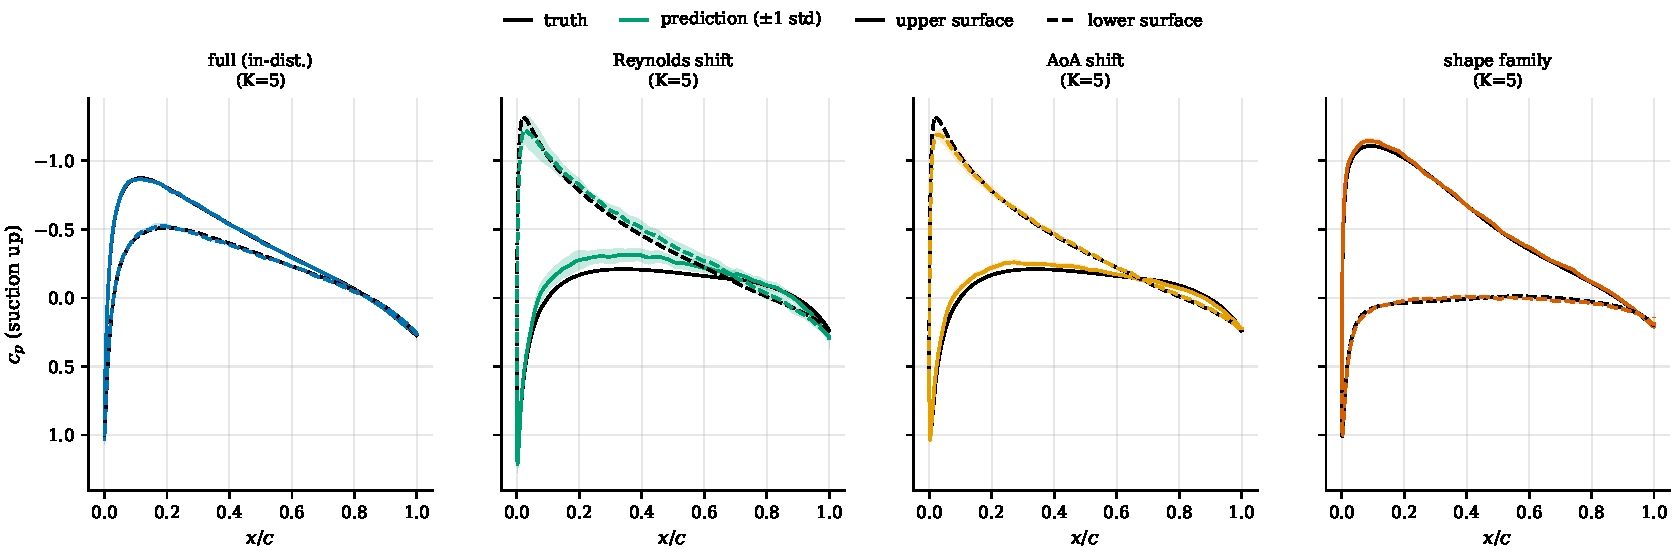
\includegraphics[width=\figwidthfull]{figures/fig02_cp_profiles.pdf}
  \caption{\Mtrans{} surface $\cp$, prediction versus truth, on one
           representative test simulation per split (full, Reynolds shift,
           AoA shift, shape family), upper and lower surface shown separately
           (solid/dashed), $\cp$ axis inverted (suction up, the aerodynamics
           convention). The shaded band is the $K=5$ deep-ensemble
           $\pm 1$ standard deviation. In distribution the ensemble mean is
           visually indistinguishable from truth and the band is a hairline;
           under Reynolds and AoA shift the mean develops a systematic
           offset near the suction peak and the band widens but (exactly
           the pattern behind \S\ref{sec:results_calibration}'s coverage
           degradation) not enough to keep the truth inside it; under
           shape-family shift (a new NACA digit family, same flow regime) the
           fit stays close and the band stays narrow, consistent with
           \splitname{shape5} being the mildest single-axis shift for every
           architecture (\S\ref{sec:results_ood}).}
  \label{fig:cp_profiles}
\end{widefigure}

\begin{widefigure}
  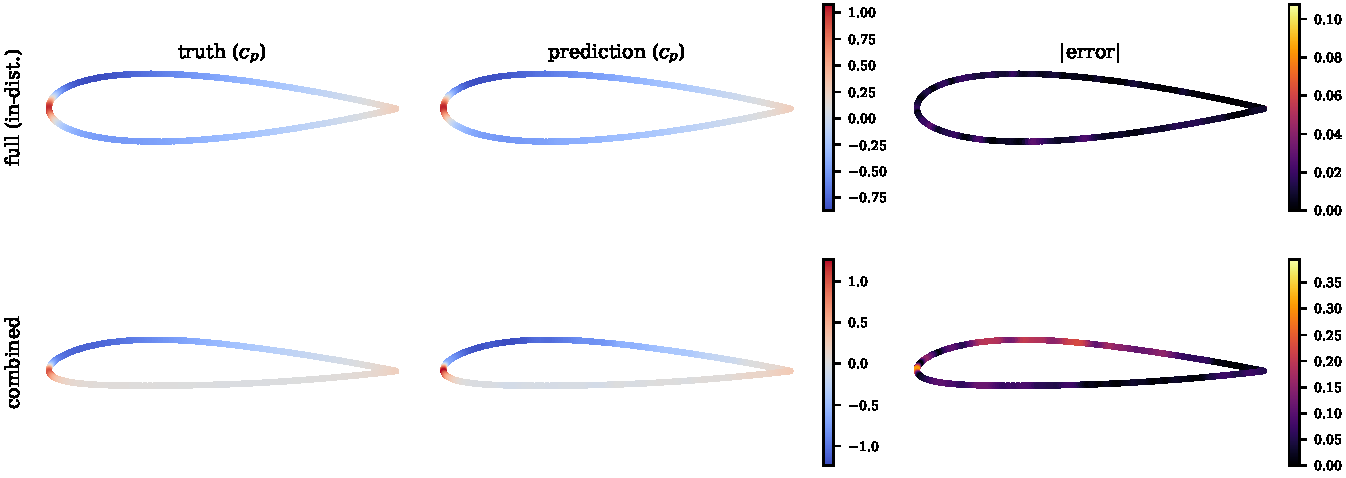
\includegraphics[width=\figwidthfull]{figures/fig03_surface_fields.pdf}
  \caption{\Mtrans{} surface $\cp$ scattered on the airfoil contour: truth,
           prediction, and absolute error (truth and prediction share one
           colour scale per row) for one in-distribution simulation
           (\splitname{full}) and one on the hardest shift
           (\splitname{combined}, shape and Reynolds shifted together), seed
           0. The error is visibly concentrated near the leading edge, where
           the combined-shift suction peak is most mispredicted.}
  \label{fig:car_surfaces}
\end{widefigure}

\subsection{Out-of-distribution}
\label{sec:results_ood}

Figure~\ref{fig:error_vs_shift} and Table~\ref{tab:ood} give the full
$3\times6$ grid (three models, six splits). The hierarchy is consistent and
physical at the extremes, for every architecture: \splitname{full} is easiest
and \splitname{combined} is hardest, and \splitname{shape5} and
\splitname{scarce} sit as the two mildest single-axis shifts, in that order.
The two remaining single-axis shifts, \splitname{reynolds} and \splitname{aoa},
are consistently the two \emph{hardest} single-axis splits but do not settle
into one fixed order between them: \Mfno{} and \Mtrans{} both find
\splitname{aoa} harder than \splitname{reynolds}, while \Mgnn{} finds the
reverse. We report this rather than round it into a clean ranking; it is a
genuine architecture-dependent disagreement about which axis hurts more,
sitting inside an otherwise architecture-independent hierarchy. \Mtrans{}
degrades from $0.019$ (\splitname{full}) to $0.139$ (\splitname{combined}), a
$7.5\times$ increase; \Mgnn{} degrades from $0.075$ to $0.270$, only
$3.6\times$: the weaker in-distribution model is, in relative terms,
\emph{more} robust to shift, so ranking by in-distribution accuracy alone
would misorder the architectures for a deployment that includes shift.

Notably this field-error ordering does not track the shift-magnitude ordering
of \S\ref{sec:protocol}: \splitname{shape5} carries the single largest
per-axis $\shift$ in the whole study ($\bar\shift = 1.00$ by construction)
while being the mildest single-axis shift for every model, and the
flow-regime shifts ($\bar\shift = 0.42$ and $0.23$) are the two hardest. A
purely geometric shift measure and the models' actual difficulty ranking
disagree, and the natural explanation is physical rather than statistical:
$\aoa$ and $\Rey$ shift move the flow toward conditions (higher effective
angle of attack, different boundary-layer character) that can cross into a
qualitatively new regime, whereas a new NACA digit family at the same $\Rey$
and $\aoa$ is still an attached-flow problem the model has seen the physics
of, just not the exact shape. These models interpolate within a flow regime
and degrade gracefully doing so, but degrade sharply once the physics itself
changes character. This reading rests on the aggregate split numbers plus the
domain knowledge that the \splitname{aoa} test range crosses
$\aoa\approx12$--$15\degrees$, close to typical NACA-section stall onset at
these Reynolds numbers; a per-simulation separation indicator would make it
precise and is left as follow-up.

On head-route $\Cd$ rank correlation the between-model gap stays below
$0.01$ on five of the six splits and peaks at $0.03$ on \splitname{reynolds}
(where \Mtrans's seeds spread most), while the between-split swing for a
single model reaches $0.05$ ($0.999\to0.94$); shift moves the ranking metric
more than architecture does, everywhere. The ridge baseline is, again, the
uncomfortable honest number: $\rho_s\in[0.83,0.90]$ across all six splits,
meaning a 29-parameter linear model captures most of the head-route
$\Cd$-ranking signal that these $\sim$1.3\,M-parameter models deliver.

The \textbf{integrated} drag ranking is the sharper counterpoint. Ranking test
cases by $\Cdint$ (drag obtained by integrating the \emph{predicted} field,
seed means as in the tables) gives $\rho_s = 0.89$ (\Mtrans), $0.83$ (\Mfno)
and $0.36$ (\Mgnn) on \splitname{full}, and collapses to $0.28$, $-0.02$ and
$-0.28$ respectively on \splitname{combined}. So the field-consistent route
ranks drag \emph{no better than ridge} for the best architecture in
distribution and far worse for the graph net, and fails entirely under the
combined shift. Any ``beats ridge'' statement in this paper is therefore a
head-route statement; the drag implied by the predicted physics does not beat
ridge. This is Gap~1 landing hard: the models learn a good drag regressor and
a good field, but not a field whose integral \emph{is} that drag, which is
exactly what \S\ref{sec:results_consistency} quantifies.

\begin{widefigure}
  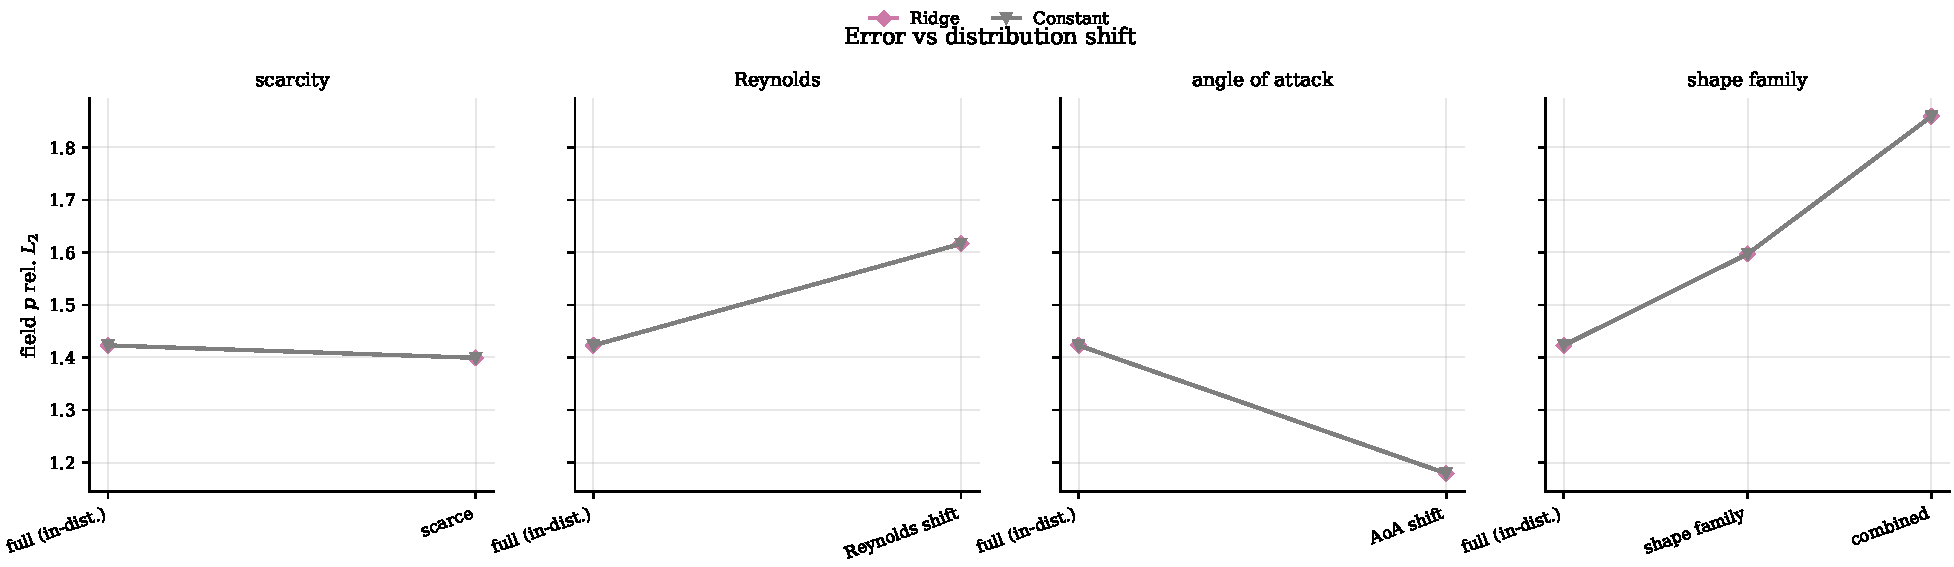
\includegraphics[width=\figwidthfull]{figures/fig04_error_vs_shift.pdf}
  \caption{Error versus distribution shift, one panel per OOD axis (scarcity,
           Reynolds, angle of attack, shape family/combined), one line per
           model, splits ordered along each axis; seed means over the
           committed core runs. Field relative $L_2$ on surface pressure.}
  \label{fig:error_vs_shift}
\end{widefigure}

\begin{widetable}
  \begin{table}[t]
\centering
\caption{Out-of-distribution field $p$ rel-$L_2$ by split.}
\label{tab:ood}
\begin{tabular}{lrrrrrr}
\toprule
model & full (in-dist.) & scarce & Reynolds shift & AoA shift & shape family & combined \\
\midrule
M1 GNN & 0.0737 & 0.154 & 0.223 & 0.188 & 0.13 & 0.27 \\
M2 SDF-FNO & 0.0257 & 0.0832 & 0.0979 & 0.111 & 0.0641 & 0.153 \\
M3 Transolver & \textbf{0.0174} & \textbf{0.0666} & \textbf{0.0773} & \textbf{0.109} & \textbf{0.0546} & \textbf{0.139} \\
Ridge & 1.42 & 1.4 & 1.62 & 1.18 & 1.6 & 1.86 \\
Constant & 1.42 & 1.4 & 1.62 & 1.18 & 1.6 & 1.86 \\
\bottomrule
\end{tabular}
\end{table}

\end{widetable}

\subsection{Consistency}
\label{sec:results_consistency}

The absolute FSC numbers in Table~\ref{tab:indist} look small only because
$\Cd$ itself is $\sim$0.01. As a fraction of the true drag (median \FSCrel),
the coefficient head and the integrated field disagree by $\approx5\%$
(\Mtrans), $7\%$ (\Mfno) and $24\%$ (\Mgnn) already in distribution, rising to
$\approx37\%$, $51\%$ and $115\%$ on \splitname{combined}. The two ``drags'' a
single model reports are tens of percent apart, and further apart the more it
extrapolates: that is why the integrated ranking in \S\ref{sec:results_ood} is
so much weaker than the head ranking.

Pooled across all 58 committed core cells (three models, six splits, all
seeds), \FSCrel{} on $\Cd$ correlates strongly with field relative $L_2$
(Pearson $r=0.89$, Spearman $\rho=0.87$): both quantities respond to the same
underlying cause, distribution shift. That pooled correlation, however, is
mostly a statement about shift, not about the models: holding the split fixed,
\Mtrans{} is both the most accurate and the most self-consistent model on
\splitname{full}, \splitname{scarce}, \splitname{shape5} and
\splitname{combined}. On \splitname{aoa}, however, \Mfno{} is the more
self-consistent model (seed-mean FSC $0.0034$ vs.\ $0.0040$) even though
\Mtrans{} remains the more accurate one in field norm; on \splitname{reynolds}
the two are statistically tied at seed means ($0.0056$ vs.\ $0.0055$; seed~0
alone puts \Mfno{} ahead there, but the seed means do not support it). That is
a concrete instance of the hypothesis this metric is meant to test: the
field-error leaderboard and the consistency leaderboard disagree, and they
disagree on a flow-regime shift, exactly where a designer relying on the
field-best model's reported drag would care most.
\FSCrel{} also grows from \splitname{full} to \splitname{combined} at least as
fast as the field error it accompanies ($4.9\times$ vs.\ $3.6\times$ for
\Mgnn, $6.9\times$ vs.\ $5.9\times$ for \Mfno, $8.0\times$ vs.\ $7.5\times$
for \Mtrans), so self-consistency is an equally or more sensitive shift
indicator than the field metric, while needing no ground truth: exactly what
makes it usable as a label-free OOD flag and as an input to the acquisition
score of \S\ref{sec:activelearning}.

\begin{figure}[t]
  \centering
  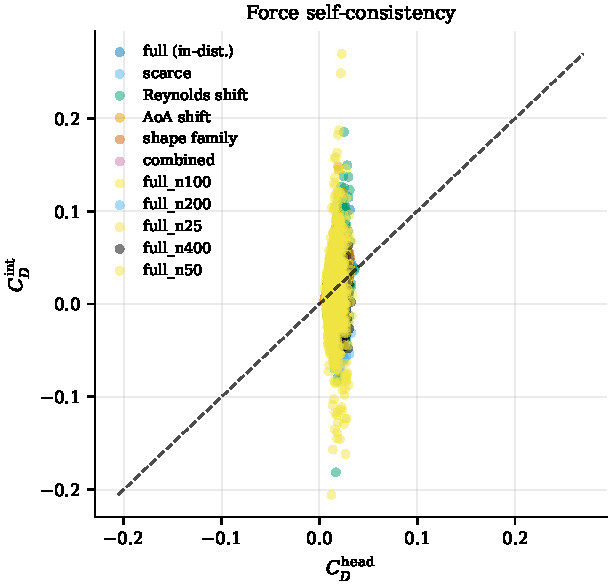
\includegraphics[width=\figw]{figures/fig05_fsc_scatter.pdf}
  \caption{Force self-consistency: $\Cdint$ against $\Cdhead$, one point per
           test simulation pooled over all three models, coloured by split,
           against the identity line (axes zoomed to the central 99\% of the
           data). Distance from the identity line is \FSC; the vertical spread
           at fixed $\Cdhead$ is the integrated route disagreeing with the
           head it shares a backbone with.}
  \label{fig:fsc_scatter}
\end{figure}

\begin{widefigure}
  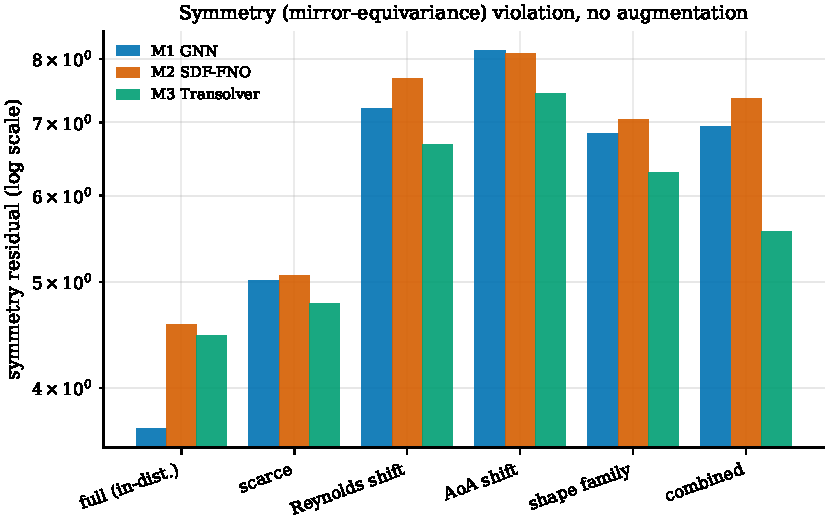
\includegraphics[width=\figwidthfull]{figures/fig10_symmetry.pdf}
  \caption{Symmetry (mirror-equivariance) residual per model, by split; no
           augmentation is applied in any run reported here
           (\S\ref{sec:models}). The residual grows from \splitname{full} to
           \splitname{aoa} for every architecture and never approaches zero,
           confirming that none of the three encodings is built to be
           equivariant to reflection; \Mtrans{} is consistently the least
           violating, \Mgnn{} and \Mfno{} track each other closely. Read
           magnitudes with the reflected-camber caveat of
           \S\ref{sec:protocol}; the growth under shift is the robust signal.}
  \label{fig:symmetry}
\end{widefigure}

\subsection{Calibration}
\label{sec:results_calibration}

Table~\ref{tab:calibration} and Figures~\ref{fig:reliability}--\ref{fig:width_dists}
report split-conformal calibration of the integrated drag band $\Cdint$ at
nominal 80/90/95\%, matched (calibrate and test on the same split's own sets)
and transfer (calibrate on \splitname{full}, deploy on the shifted split).
Ensembles cover \{\splitname{full}, \splitname{reynolds}, \splitname{aoa},
\splitname{shape5}\}: $K=5$ for \Mfno{} and \Mtrans, $K=3$ for \Mgnn{} (the
$k$NN graph net costs $7$--$8\times$ more per run, so it gets a smaller
ensemble by design). One wording caveat up front: each split's calibration set
is carved from that split's own \emph{training} pool, so ``matched'' means a
like-distributed calibration set is available, the optimistic case; it is not
recalibration on labelled cases from the shifted deployment itself, which is
not run here.

On a calibration set of $n$ simulations disjoint from train and test, with
normalised nonconformity score
$\score_j = \abs{y_j - \ubar(\bx_j)} / (\sigmahat(\bx_j) + \eps)$ and $\qhat$ its
$\lceil (n+1)(\nomlevel) \rceil / n$ empirical quantile,
\begin{equation}
  \conf(\bx) = \left[ \ubar(\bx) - \qhat\,\sigmahat(\bx),\;
                      \ubar(\bx) + \qhat\,\sigmahat(\bx) \right],
\end{equation}
which satisfies $\Prob(y \in \conf(\bx)) \geq \nomlevel$ when calibration and
test data are exchangeable. An \emph{absolute} score
($\score_j = \abs{y_j - \ubar(\bx_j)}$, a fixed-width band) is calibrated in
parallel, and the contrast between the two matters below. Two granularities are
calibrated separately: per-simulation coefficient intervals, where the
exchangeable unit is a whole simulation and the guarantee is clean; and
pointwise field intervals, where points within a simulation are \emph{not}
exchangeable, so we conformalise at the simulation level with a
quantile-over-points score and state the weaker interpretation rather than
implying a pointwise guarantee.

\textbf{In distribution, matched calibration is close to nominal for the two
stronger models but not automatic}: coverage at nominal 90\% is $0.955$
(\Mfno) and $0.91$ (\Mtrans), while \Mgnn{} \emph{under-covers} at $0.82$
(Wilson 95\% interval $[0.76, 0.87]$, excluding $0.90$). ``The conformal
guarantee holds in distribution'' is therefore true for two of three models
here, not all three.

\textbf{Under shift, a high coverage number can be an artifact of band width,
and the honest reading requires both columns of Table~\ref{tab:calibration}.}
The clearest case is \Mgnn{} on \splitname{reynolds}: matched coverage $0.97$
looks like a calibration win, but the normalized band behind it has mean width
$0.228$ for a $\Cd$ of $\sim$0.01, an interval $\approx23\times$ the quantity
it brackets: near-vacuous. The tight absolute-score band on the same split
covers only $0.70$, essentially unchanged from a single member, so the
ensemble did not genuinely fix the graph net under shift; it inflated the
variance-scaled interval. We report both scores rather than quote the
flattering one. The stronger models fail elsewhere: \Mfno{} under-covers on
\splitname{shape5} ($0.763$ at nominal 90, its worst split), the shift
\S\ref{sec:results_ood} found mildest for field accuracy but evidently not for
calibration; \Mtrans{} is the most consistently calibrated of the three
(matched coverage $0.87$--$0.95$ everywhere) but also dips on
\splitname{shape5} ($0.867$).

\textbf{ECE degrades most on the deployment-relevant absolute-score bands.}
On the absolute score, ECE jumps $6$--$10\times$ from \splitname{full} to the
flow-regime shifts (\Mgnn{} $0.022\to0.16$, \Mfno{} $0.047\to0.27$, \Mtrans{}
$0.040\to0.44$). Table~\ref{tab:calibration}'s ECE column reports the
normalized-score ECE, which moves far less (e.g.\ \Mtrans{} $0.007\to0.035$)
precisely because the normalized band widens with the ensemble variance: the
same band-width effect as the coverage row, stated here so the table cannot be
over-read.

\textbf{Matched versus transfer calibration does not order cleanly.} Naively,
matched calibration (the split's own, in-principle-exchangeable calibration
set) should be the safer choice. The data does not cooperate: on
\splitname{shape5}, transfer beats matched for \Mfno{} ($0.847$ vs.\ $0.763$)
but loses to it for \Mgnn{} ($0.818$ vs.\ $0.863$) and \Mtrans{} ($0.814$
vs.\ $0.867$); on \splitname{reynolds} the normalized matched numbers exceed
transfer for \Mgnn{} and \Mtrans{} while \Mfno{} orders the other way
($0.895$ vs.\ $0.940$). No single choice of calibration set is reliably safer
once exchangeability has broken: evidence that the failure is structural (the
score's relationship to error has genuinely changed under shift) rather than
a fixable artifact of which calibration set was used.

\textbf{Interval width widens under shift for every model
(Figure~\ref{fig:width_dists}), but under-compensates.} $\Cdint$ band width at
nominal 90\% grows from \splitname{full} to the harder splits (e.g.\ \Mfno{}
$0.0085\to0.022$, \Mtrans{} $0.0056\to0.021$ on \splitname{reynolds}, roughly
$2.5$--$3.7\times$). That the uncertainty estimate responds to shift at all is
informative (an unresponsive score would be worse), but coverage still drops
on the same splits where width grows most, which is what ``widening honestly
but insufficiently'' looks like in a reliability diagram
(Figure~\ref{fig:reliability}).

\textbf{The conclusion, stated as plainly as the numbers allow: split
conformal prediction repairs in-distribution calibration for a well-behaved
model with a like-distributed calibration set, but its coverage guarantee is
not robust to distribution shift.} A 90\% conformal interval computed on this
study's splits must not be read as a 90\% probability statement once the input
has moved outside the calibration distribution: under a flow-regime shift the
deployment-relevant absolute-score coverage can be as low as $0.70$ in this
study, and a high normalized-score coverage may be reporting nothing more than
a very wide band. Practically, a conformal interval should be trusted only for
inputs a label-free monitor (such as \FSC, \S\ref{sec:results_consistency})
has flagged as in-distribution, and a reported coverage should always be read
next to its interval width.

\begin{widetable}
  \begin{table}[t]
\centering
\caption{Split-conformal calibration of the integrated drag band ($C_D^{\mathrm{int}}$): empirical coverage, mean interval width and ECE. Matched calibrates on the split's own cal set; transfer (tr) calibrates on \texttt{full}'s cal.}
\label{tab:calibration}
\begin{tabular}{llrrrrrr}
\toprule
model & split & cov@.8 & cov@.9 & cov@.95 & cov@.9 (tr) & width@.9 & ECE \\
\midrule
M1 GNN & full (in-dist.) & 0.735 & 0.82 & 0.92 & 0.82 & 0.0332 & 0.0583 \\
M1 GNN & shape family & 0.718 & 0.863 & 0.959 & 0.818 & 0.0467 & 0.0426 \\
M1 GNN & Reynolds shift & 0.933 & 0.966 & 0.972 & 0.917 & 0.228 & 0.0737 \\
M1 GNN & AoA shift & 0.816 & 0.893 & 0.929 & 0.893 & 0.0575 & 0.015 \\
M2 SDF-FNO & full (in-dist.) & 0.885 & 0.955 & 0.98 & 0.955 & 0.00854 & 0.0567 \\
M2 SDF-FNO & shape family & 0.648 & 0.763 & 0.879 & 0.847 & 0.00731 & 0.12 \\
M2 SDF-FNO & Reynolds shift & 0.75 & 0.895 & 0.938 & 0.94 & 0.0218 & 0.0224 \\
M2 SDF-FNO & AoA shift & 0.913 & 0.944 & 0.974 & 0.929 & 0.0159 & 0.0605 \\
M3 Transolver & full (in-dist.) & 0.805 & 0.91 & 0.955 & 0.91 & 0.00562 & 0.00667 \\
M3 Transolver & shape family & 0.793 & 0.867 & 0.908 & 0.814 & 0.00746 & 0.0275 \\
M3 Transolver & Reynolds shift & 0.76 & 0.938 & 0.978 & 0.915 & 0.021 & 0.0351 \\
M3 Transolver & AoA shift & 0.821 & 0.949 & 0.959 & 0.949 & 0.0198 & 0.0265 \\
\bottomrule
\end{tabular}
\end{table}

\end{widetable}

\begin{widefigure}
  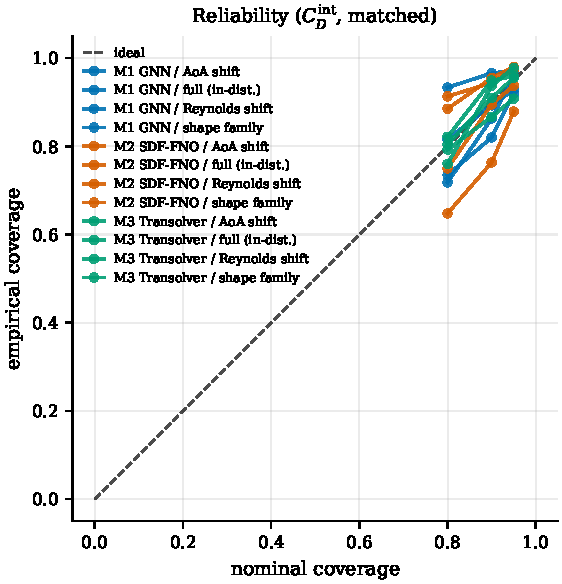
\includegraphics[width=\figwidthfull]{figures/fig06_reliability.pdf}
  \caption{Reliability of the matched-calibration $\Cdint$ band, one panel per
           model, coloured by split, largest available $K$ per model ($K=3$
           \Mgnn, $K=5$ otherwise): empirical versus nominal coverage at
           80/90/95\%. Curves below the diagonal under-cover.}
  \label{fig:reliability}
\end{widefigure}

\begin{figure}[t]
  \centering
  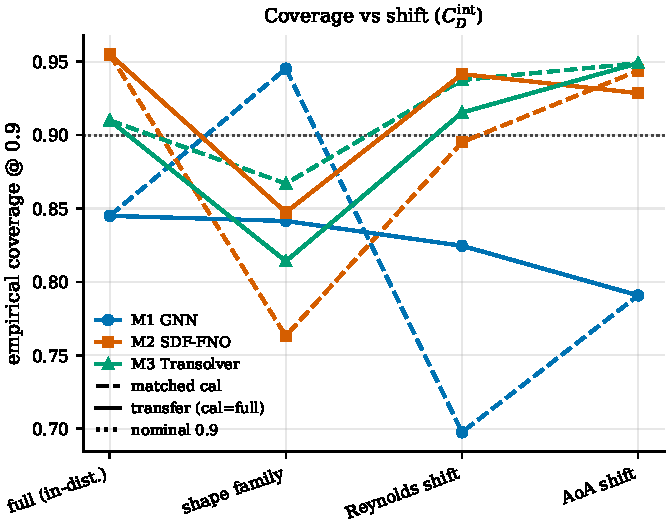
\includegraphics[width=\figw]{figures/fig07_coverage_vs_shift.pdf}
  \caption{Empirical coverage at nominal 90\% against split, matched (dashed)
           versus transfer-calibrated on \splitname{full} (solid), normalized
           score. Neither calibration choice reliably dominates once the split
           shifts, and \Mgnn's high \splitname{reynolds} point rides on a
           near-vacuous band width (\S\ref{sec:results_calibration}).}
  \label{fig:coverage_vs_shift}
\end{figure}

\begin{widefigure}
  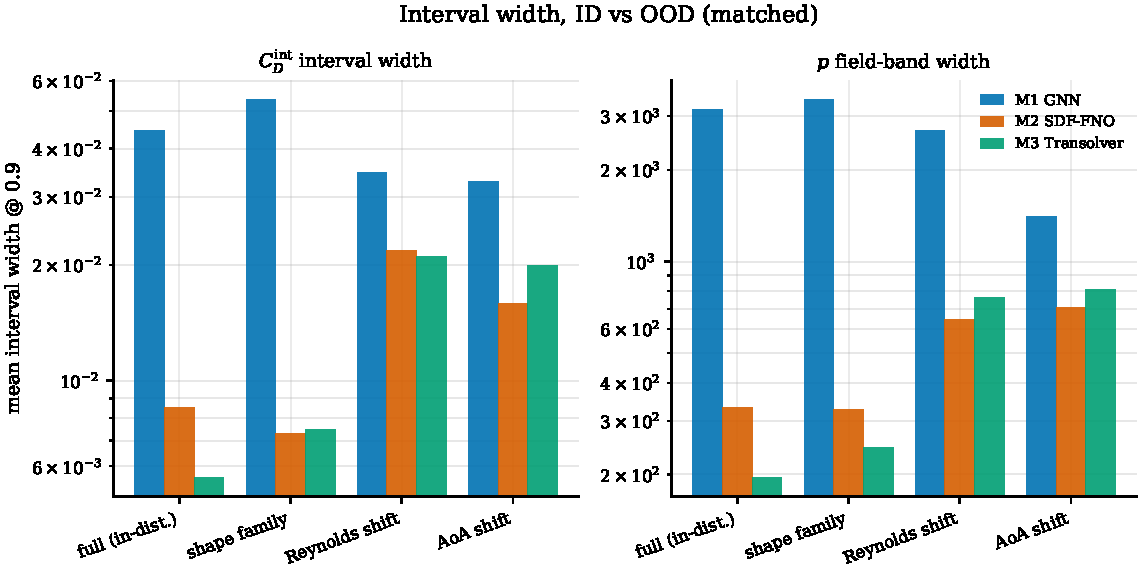
\includegraphics[width=\figwidthfull]{figures/fig08_interval_width.pdf}
  \caption{Interval-width distributions, in-distribution versus OOD, matched
           calibration: mean interval width at nominal 90\%, per model and
           split, for the $\Cdint$ coefficient band and the pointwise field
           band (log scale; the field band is in kinematic-pressure units).
           Widths grow from \splitname{full} outward for every model, but, as
           Table~\ref{tab:calibration} and Figure~\ref{fig:coverage_vs_shift}
           show together, not by enough to keep coverage at nominal under
           shift.}
  \label{fig:width_dists}
\end{widefigure}

\subsection{Data efficiency and cost}
\label{sec:results_efficiency}

All three models were retrained at training-set sizes
$\{25, 50, 100, 200, 400\}$, three seeds each (45 runs), with the full-700
point reused from the core grid: Figure~\ref{fig:efficiency}(a). Two things
are worth the reader's attention. First, \textbf{\Mtrans{} is the most
accurate at every size}, including 25 airfoils (field $p$ rel-$L_2$ $0.271$
vs.\ $0.292$ for \Mgnn{} and $0.325$ for \Mfno): the transformer's advantage
is not a large-data artifact. Second, \textbf{the \Mfno-vs-\Mgnn{} order
crosses}: the graph net is the better of the two in the scarce regime
($n=25$: $0.292$ vs.\ $0.325$; $n=50$: $0.217$ vs.\ $0.232$) and \Mfno{}
overtakes it only around $n\approx70$--$100$, after which its spectral route
scales much faster (at $n=700$: $0.026$ vs.\ $0.075$). The crossing is clear
on the seed means; in seed-noise terms the $n=50$ gap is $\approx1.6$--$2.4$
standard deviations over three seeds while the $n=25$ gap is within one, so
the statement ``\Mfno{} is the most data-hungry of the three below
$\sim$100 airfoils'' is solid from $n=50$ up and indicative at $n=25$. The
clean \Mtrans{} $>$ \Mfno{} $>$ \Mgnn{} hierarchy of
\S\ref{sec:results_id} is therefore a large-data statement, and a
single-budget ranking under-specifies method choice for data-scarce practice.

The cost axis (Figure~\ref{fig:efficiency}(b)) makes the deployment reading direct:
at the full budget \Mgnn{} is Pareto-dominated, costing $2.4$--$3.2$ GPU-h
across seeds (mean $2.9$) to
train against \Mfno's $0.36$\,h and \Mtrans's $0.41$\,h (the $k$NN
reconstruction on every forward pass dominates its cost) while also being the
least accurate. The efficient frontier is \Mtrans{} and \Mfno; \Mgnn's appeal
below $n\approx100$ (above) is the one place this study found it earning its
cost.

\begin{widefigure}
  \begin{minipage}{0.48\figwidthfull}\centering
    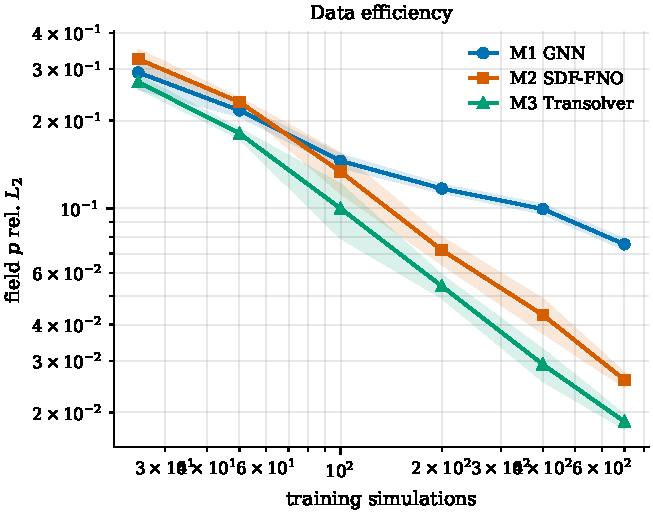
\includegraphics[width=\linewidth]{figures/fig09_data_efficiency.pdf}
  \end{minipage}\hfill
  \begin{minipage}{0.48\figwidthfull}\centering
    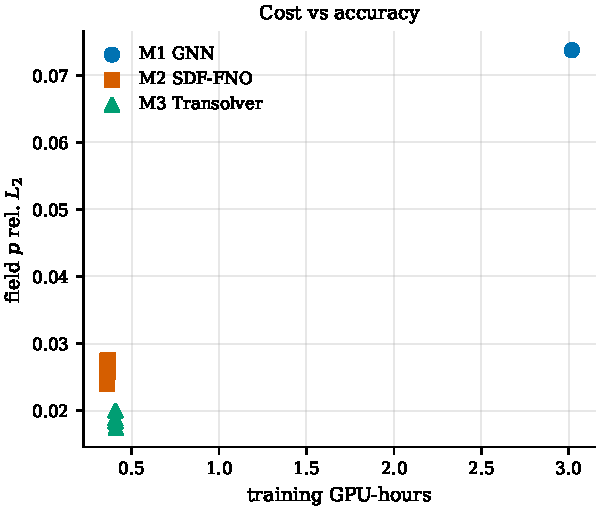
\includegraphics[width=\linewidth]{figures/fig12_cost_accuracy.pdf}
  \end{minipage}
  \caption{Data efficiency and the cost--accuracy trade-off. (a) Data
           efficiency: field error against training-set size, log-log, seed
           bands shaded. The \Mfno/\Mgnn{}
           curves cross around $n\approx70$--$100$ training simulations;
           \Mtrans{} leads everywhere. (b) Cost versus accuracy at the full
           training budget.}
  \label{fig:efficiency}
\end{widefigure}

\subsection{Ablations}
\label{sec:results_ablations}

Table~\ref{tab:ablations} reports the two ablation axes run for this version
(seed 0). \textbf{Geometry conditioning for \Mfno:} the binary occupancy mask
is the worst encoding on both splits ($0.029$ in distribution, $0.073$ on
\splitname{shape5}), SDF is best in distribution ($0.026$), and SDF plus
surface normals gives the best out-of-family accuracy ($0.061$ vs.\ $0.064$
for SDF alone). This reproduces the published finding that SDF beats a mask
\citep{rabeh2025benchmarking} and adds that normals help specifically under
shape-family shift. \textbf{Force-consistency loss for \Mgnn:} switching
$\lamF$ on cuts FSC by $4\times$ in distribution ($0.0053\to0.0013$) and
$3\times$ on \splitname{combined}, while \emph{worsening} in-distribution
field accuracy ($0.074\to0.104$): the physics term shrinks exactly the
residual it penalises and buys self-consistency, not accuracy. This is the
predicted negative result, reported as found. The ensemble-size axis is
implicit in the $K\in\{1,3,5\}$ conformal reports of
\S\ref{sec:results_calibration} (the \Mgnn{} $K=1\to3$ comparison there is
its most instructive data point); the augmentation ablation for the symmetry
residual was cut from this version's scope.

\begin{widetable}
  % Table 4 -- ablations (see tab4_ablation.md for the readable form)
% M2 conditioning and M1 force-loss; values are field p rel-L2 / FSC.

\end{widetable}

% =====================================================================
\section{Active learning with solver verification}
\label{sec:activelearning}
% =====================================================================

This section turns \FSC{} and ensemble spread from diagnostics into a use: a
label-free score that picks which of many un-simulated candidates is worth the
cost of a new CFD run, verified against a solver (Ansys Fluent 2021~R1) that
did not generate the training data. The outcome is stated honestly up front:
the score concentrated its picks on the corner of the pool where the steady
operator the surrogate learned mostly has no settled solution, so the
quantitative comparison is a qualitative external check on the solvable
subset, not a large-sample statistical test.

\subsection{Acquisition}
The pool is a parametric family of NACA 4- and 5-digit sections crossed with a
grid of $(\Rey, \aoa)$: 630 candidates, $\Rey\in\{2,\dots,7\}\times10^6$,
$\aoa\in\{-6,0,6,12,18\}\degrees$, none coinciding with a training case. Each
candidate is scored
\begin{equation}
  \acq(\geom,\cond) = \underbrace{\sigmahat_{\Cd}(\geom,\cond)}_{\text{spread}}
    + \betaacq \underbrace{\FSC(\geom,\cond)}_{\text{self-inc.}}
    + \gammaacq \underbrace{\Losssym(\geom,\cond)}_{\text{sym.\ viol.}},
\end{equation}
all three normalised to unit variance over the pool, with
$\betaacq = \gammaacq = 1$. The top-$k$ are selected subject to greedy
farthest-point diversity in normalised design space. Three arms of $k=8$:
acquisition, pure ensemble variance, and random. Scorer: the \Mtrans{} $K=5$
\splitname{full} ensemble.

Figure~\ref{fig:active_learning}(a) shows the result before any solver runs: the
acquisition and variance arms place \textbf{all 16 of their picks at
$\aoa=18\degrees$}, the top of the pool grid and well past both the training
range ($12.5\degrees$) and the dataset's own envelope ($\sim$15$\degrees$),
while the random arm spreads across the envelope. Two disclosures qualify
this. First, the score is built from the \emph{integrated} $\Cd$ on the
synthetic pool contour, and that representation carries a large artifact off
the real mesh (pool $\sigma_{\Cd}\approx0.15$--$0.24$ and
$\FSC\approx0.08$--$0.31$ for a $\Cd$ of $\sim$0.03, versus $\sim$0.001 on
real meshes in distribution; the root cause was not isolated and is logged as
open). Second, the pool grid overshoots the training envelope on both axes by
construction, so the extreme corner was nearly guaranteed to top a ranking
that rewards extrapolation. The defensible claim is therefore that the
label-free score \textbf{flags the out-of-envelope corner}: it detects
extrapolation, which here coincides with hard physics, and the solver runs
below test what that is worth.

\begin{widefigure}
  \begin{minipage}{0.48\figwidthfull}\centering
    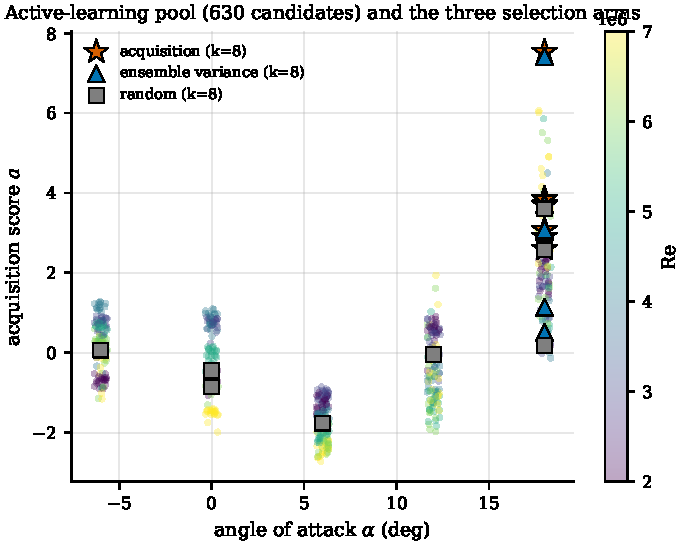
\includegraphics[width=\linewidth]{figures/fig11_active_pool.pdf}
  \end{minipage}\hfill
  \begin{minipage}{0.48\figwidthfull}\centering
    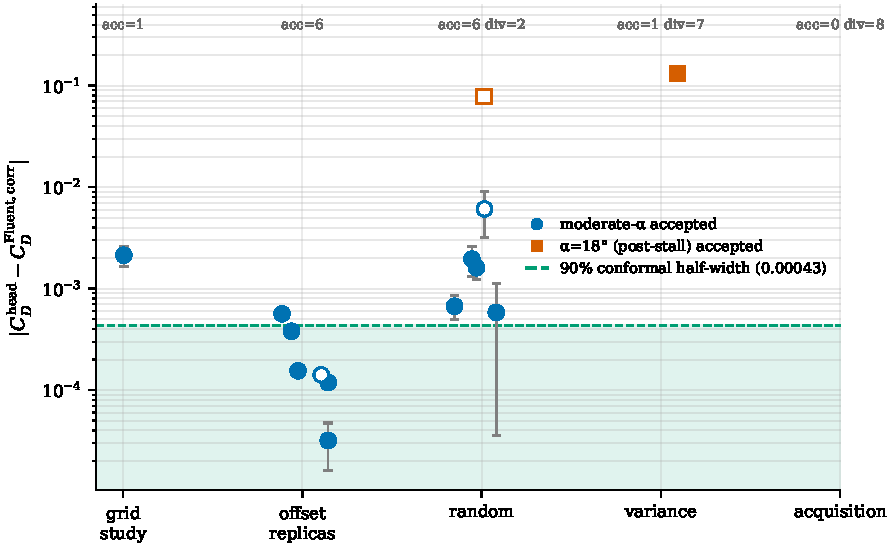
\includegraphics[width=\linewidth]{figures/fig11_active_verify.pdf}
  \end{minipage}
  \caption{Active learning: (a) the 630-candidate pool against $\aoa$,
           coloured by $\Rey$, with the three $k{=}8$ arms marked; acquisition
           and pure-variance selection agree with each other (all 16 picks at
           $\aoa=18\degrees$) and disagree with random. (b) \Mtrans{}
           $|C_D|$ error against the offset-corrected Fluent value on the
           accepted set, by arm and regime; the annotations count accepted
           (acc) and non-settling (div) cases per arm, and the shaded band is
           the 90\% conformal half-width from the \splitname{full}
           calibration study.}
  \label{fig:active_learning}
\end{widefigure}

\subsection{Solver setup, grid independence, and the solver offset}
\label{sec:fluent_setup}
Every selected case runs as 2D steady incompressible RANS on a parameterised
structured C-grid, wall-resolved ($y^+_{\max}\leq1.1$ on every accepted
case), with Spalart--Allmaras \citep{spalart1992sa} as the like-for-like
closure (matching AirfRANS's own generation) and $k$--$\omega$ SST
\citep{menter1994sst} run per case for a model-sensitivity spread. A
three-level grid study on NACA0012 at $\Rey=3\times10^6$, $\aoa=5\degrees$
(18{,}796 / 43{,}008 / 96{,}768 cells) gives $C_D$ changing $3.3\%$ from L1
to L2 and $0.003\%$ from L2 to L3 with $C_L$ within $0.3\%$ and $y^+<1$
everywhere: grid-independent at L2, the level every production case uses
(Appendix~\ref{app:cfd} reports the Celik GCI \citep{celik2008gci,
roache1994perspective} and the sanity checks). The SA-SST $C_D$ spread at L2
is $1.5\%$.

Because Fluent and the OpenFOAM setup behind AirfRANS differ in solver,
discretisation and mesh topology, six AirfRANS \emph{test} simulations were
replicated in Fluent (geometry gate: maximum nearest-neighbour distance to
the cached surface below $8\times10^{-5}$ chords) to measure the solver
offset before interpreting any surrogate-versus-Fluent gap
(Table~\ref{tab:fluent_offset}). On SA, $\bar{\delta}_{C_D} = +0.00090$
($s = 0.00034$, $n=6$; every replica positive, $5.3$--$13\%$ of $C_D$), and
$\bar{\delta}_{C_L} = +0.0122$. Crucially, the per-case SA-SST spread
($0.00003$--$0.0005$) is \emph{smaller} than the offset, so at these angles
the solver difference, not the turbulence model, is the dominant systematic;
the mean SA offset is subtracted from every Fluent $C_D$ before comparison.
The replica scatter $s = 0.00034$ is itself as large as the surrogates'
in-distribution $C_D$ MAE ($\sim$0.00012--0.00014), a solver-side floor that
the comparison below cannot go beneath.

\begin{widetable}
  \caption{Solver offset: six AirfRANS test simulations re-solved in Fluent (SA, grid level L2). $\delta C_D = C_D^{\mathrm{Fluent}} - C_D^{\mathrm{AirfRANS}}$; every replica reads high, so the mean offset $\bar{\delta}_{C_D}$ is subtracted before any surrogate comparison.}
\label{tab:fluent_offset}
\small
\setlength{\tabcolsep}{4pt}
\begin{tabular}{lrrrrrr}
\toprule
replica & $C_D^{\mathrm{AF}}$ & $C_L^{\mathrm{AF}}$ & $C_D^{\mathrm{SA}}$ & $C_D^{\mathrm{SST}}$ & $\delta C_D$ & rel.\ $\delta C_D$ \\
\midrule
offset\_4\_naca2710\_am1p6 & 0.009226 & 0.0513 & 0.009719 & 0.009553 & 0.000493 & 0.0534 \\
offset\_1\_naca0016\_a2p4 & 0.009702 & 0.251 & 0.01048 & 0.01019 & 0.00078 & 0.0804 \\
offset\_2\_naca0109\_a8p6 & 0.01151 & 0.926 & 0.01301 & 0.01304 & 0.0015 & 0.13 \\
offset\_6\_naca5\_17\_a0p9 & 0.009805 & 0.219 & 0.01082 & 0.01032 & 0.00101 & 0.103 \\
offset\_3\_naca2211\_a3p3 & 0.009052 & 0.607 & 0.009919 & 0.009786 & 0.000867 & 0.0958 \\
offset\_5\_naca0010\_a3p8 & 0.008058 & 0.419 & 0.00881 & 0.008599 & 0.000752 & 0.0933 \\
\midrule
mean $\pm$ s (SA, n=6) & & & & & +0.0009 $\pm$ 0.00034 & \\
\bottomrule
\end{tabular}

\end{widetable}

\subsection{Campaign outcome}
\label{sec:fluent_outcome}
Of the 33 cases run (3 grid levels, 6 replicas, 24 arm picks), the grid trio,
all 6 replicas, 4 low-$\aoa$ random picks and (on retry) the $\aoa=12\degrees$
random pick converged or reached a clean quasi-steady state. \textbf{All 20
first-attempt divergences sat at the aggressive corner}: the 16 acquisition-
and variance-arm picks (all $\aoa=18\degrees$), 3 random $\aoa=18\degrees$
picks, and one random $\aoa=12\degrees$ case. A conservative retry (longer
first-order start, reduced under-relaxation, no early stopping) split that
set three ways: the in-envelope $\aoa=12\degrees$ case recovered cleanly
($C_D=0.019$), confirming a settings failure rather than physics; \textbf{two
$\aoa=18\degrees$ cases genuinely settled} (the variance-arm pick, converged
$C_D=0.167$ with
drift $0.2\%$, and a random-arm case, quasi-steady $C_D=0.113$); and of the
remaining 17,
sixteen ran their
full 7000 iterations at bounded, physically plausible post-stall magnitudes
(final $C_D\approx0.06$--$0.15$) while still drifting $7$--$21\%$ over the
last 500 iterations and one errored out at iteration 725, so all 17 are
classified non-settling: past the envelope
where this steady-RANS operator has a solution to converge to. A
time-averaged URANS truth for those 17 is future work, and would compare the
surrogate to a quantity it was never trained to predict.

\subsection{Surrogate versus Fluent}
\label{sec:fluent_compare}
For every accepted case the trained ensembles were evaluated at that geometry
and condition and compared to the offset-corrected Fluent coefficient
(Table~\ref{tab:fluent_verify}; per-case rows in
Appendix Table~\ref{tab:fluent_cases}). The reported surrogate $C_D$ is the
coefficient head; the integrated route on the synthetic pool contour carries
the representation artifact disclosed above, so it is kept only as a
diagnostic. The accepted set has two regimes, and averaging them into one MAE
would hide the entire finding.

\textbf{Moderate $\aoa$ (n=12, $-6\degrees$ to $12\degrees$):} surrogate
$C_D$ error is $3$--$10\times$ its in-distribution level (MAE $0.00037$ for
\Mgnn, $0.0012$ \Mtrans, $0.0013$ \Mfno{} against in-distribution
$\sim$0.00012--0.00014), and the 90\% conformal intervals under-cover for
two of three models (\Mtrans{} $0.42$, \Mfno{} $0.33$; \Mgnn's $0.83$ rides
on its wider band, \S\ref{sec:results_calibration}). Verified against a
solver that did not generate the training data, the C3 calibration
degradation reproduces against external truth. Part of this gap is the
solver-side floor above, which is negligible against what follows.

\textbf{Post-stall (n=2, the settled $\aoa=18\degrees$ cases):} the
surrogates predict attached-flow drag ($\Chead\approx0.03$--$0.06$) where
the offset-corrected settled Fluent values are $0.113$ and $0.165$: errors of
$0.05$--$0.13$ per case, roughly $640$--$900\times$ the in-distribution MAE,
every one far outside its conformal band.

\subsection{The C4 finding}
The falsifiable claim was: cases with high acquisition score have higher
surrogate error against independent truth than randomly selected ones. The
verdict splits cleanly by half. The half that says \emph{high-score picks are
cases the surrogate fails on} is now supported with a hard number: the one
high-score ($\aoa=18\degrees$ variance-arm) pick the solver settled carries a
surrogate error orders of magnitude above the moderate-regime error level,
and the other 15
high-score picks sit where the
steady solver itself does not settle, the strongest possible form of ``the
surrogate should not be trusted here.'' (The second settled
$\aoa=18\degrees$ case belongs to the random arm and fails identically,
which cuts against the other half below.) The half that says \emph{random picks
are cases the surrogate gets right} is only partly true: on the tightly
controlled offset replicas the surrogate sits inside its band in 15 of 18
model-case pairs, but on the random arm coverage is 3/6 (\Mgnn) and 0/6
(\Mfno, \Mtrans). So the score does separate hard from easy, the conformal
bands do not survive the trip, and both statements are visible at once in
Figure~\ref{fig:active_learning}(b).

\begin{widetable}
  \caption{Surrogate vs.\ Fluent on the accepted steady set, split by regime (all cases at the grid-independent L2 level, Appendix~\ref{app:cfd}; qualitative external check, \S\ref{sec:activelearning}). Surrogate $C_D$ is the coefficient head, compared against the offset-corrected Fluent value; cov@90 is the fraction inside that model's 90\% conformal interval from the \texttt{full}-split calibration study. In-dist.\ MAE is the same model's $C_D$ MAE on the \texttt{full} test set.}
\label{tab:fluent_verify}
\providecommand{\tblfont}{\footnotesize}%
\tblfont
\setlength{\tabcolsep}{4pt}
\begin{tabular}{lrrrrrr}
\toprule
& \multicolumn{4}{c}{moderate $\alpha$ ($-6\degrees..12\degrees$)} & \multicolumn{2}{c}{post-stall ($\alpha=18\degrees$)} \\
\cmidrule(lr){2-5}\cmidrule(lr){6-7}
model & $n$ & MAE $C_D$ & ratio to in-dist. & cov@90 & $n$ & MAE $C_D$ \\
\midrule
M1 GNN & 12 & 0.00037 & 3$\times$ & 0.83 & 2 & 0.1 \\
M2 SDF-FNO & 12 & 0.0013 & 9.2$\times$ & 0.33 & 2 & 0.087 \\
M3 Transolver & 12 & 0.0012 & 10$\times$ & 0.42 & 2 & 0.11 \\
\bottomrule
\end{tabular}

\end{widetable}

% =====================================================================
\section{Discussion and limitations}
\label{sec:discussion}
% =====================================================================

Overclaiming is the single biggest risk to a paper whose subject is trust, so
this section is written to be read, not skimmed.

\paragraph{Limitations.}
\begin{itemize}\itemsep2pt
  \item \textbf{Seed counts vary by cell.} Core-grid cells on \splitname{full},
        \splitname{reynolds}, \splitname{aoa} and \splitname{shape5} carry
        3--5 seeds (Tables~\ref{tab:indist}--\ref{tab:ood} report seed mean
        $\pm$ std); \splitname{scarce} and \splitname{combined} are
        single-seed, so per-seed spread there is unknown. Ensembles are $K=5$
        for \Mfno/\Mtrans{} and $K=3$ for \Mgnn{} (a cost decision, stated in
        \S\ref{sec:results_calibration}); no ensemble exists on
        \splitname{scarce} or \splitname{combined}, so no conformal result is
        claimed there.
  \item \textbf{One dataset family, 2D only.} Everything here is AirfRANS:
        2D airfoils, incompressible RANS, Spalart--Allmaras upstream. No claim
        extends to 3D geometry, compressible flow, or other solvers.
        DrivAerNet++ remains future work (\S\ref{sec:data}).
  \item \textbf{The ``matched'' calibration is the optimistic case.} Each
        split's calibration set is carved from its own training pool
        (\S\ref{sec:results_calibration}); recalibrating on labelled cases
        from the shifted deployment itself is the practically interesting
        variant and is not run here.
  \item \textbf{The acquisition outcome is confounded by its own
        construction.} The score uses the integrated $\Cd$ on a synthetic
        pool contour that carries a large representation artifact
        (\S\ref{sec:activelearning}; root cause open), and the pool grid
        overshoots the training envelope on both axes, so ``all 16 picks at
        $\aoa=18\degrees$'' should be read as the score flagging the
        out-of-envelope corner, not as evidence that a calibrated field-level
        uncertainty located hard physics on its own.
  \item \textbf{The Fluent leg is an external check, not a statistical
        test.} Fourteen accepted cases, two of them post-stall; the solver
        offset is bounded by six replicas whose scatter ($s_{C_D}=0.00034$)
        is as large as the surrogates' in-distribution MAE and is not folded
        into the coverage test. Ten pool cases (two accepted) at
        $\Rey=7\times10^6$ run at $M\approx0.32$, past the usual
        incompressible limit; solver and surrogate are both incompressible,
        so the comparison is internally consistent, but absolute coefficients
        there carry that caveat.
  \item \textbf{The symmetry residual is a response-to-reflection indicator.}
        For cambered sections the reflected input is out-of-family
        (\S\ref{sec:protocol}), so absolute magnitudes overstate pure
        equivariance violation; the zero-camber clean test is future work.
        (The cached signed curvature fed to the reflected batch was verified
        numerically identical to recomputing it on the mirrored contour, so
        the harness itself is sound.)
  \item \textbf{Reimplementations, not the authors' code}
        (\S\ref{sec:models}): absolute numbers are not comparable with
        published ones; only the within-study comparison is meaningful.
  \item \textbf{Compute budget.} Free-tier cloud T4 sessions and a 4\,GB
        laptop GPU, 61 GPU-hours total (Appendix~\ref{app:compute}); every
        model trains exactly 400 epochs at batch 16. Rankings at a
        substantially larger budget may differ, which is exactly what the
        data-efficiency curves are for.
  \item \textbf{Single author.} No co-author caught bugs. Mitigations: the
        force integrator is gated against ground truth before anything
        downstream runs (\S\ref{sec:protocol}); split disjointness is
        asserted programmatically for every manifest; and multiple
        independent automated review passes audited the codebase and the
        results, catching real defects that were fixed before this text was
        written (a normalisation leak across splits, a table aggregation that
        mixed ablation runs into core cells, and a divergence classifier that
        misread the iteration-1 startup transient; all disclosed in the
        repository's decision log).
\end{itemize}

\paragraph{Negative and mixed results, reported as found.} The ridge baseline
(29 parameters, zero training cost) is competitive on head-route $\Cd$ rank
correlation across every split ($\rho_s\in[0.83,0.90]$), and the integrated
drag ranking of the best neural model does not beat it at all
(\S\ref{sec:results_ood}). The architecture that wins on field accuracy is not
always the most internally self-consistent: \Mfno{} out-consistents \Mtrans{}
on the AoA shift and ties it on the Reynolds shift
(\S\ref{sec:results_consistency}). The
force-consistency training term buys self-consistency, not accuracy
(\S\ref{sec:results_ablations}). Matched-versus-transfer conformal
calibration does not order cleanly (\S\ref{sec:results_calibration}). The
\Mgnn{} ensemble upgrade ($K=1\to3$) raised its normalized shifted coverage
without moving the absolute-score coverage: a band-width effect, not a
calibration gain, disclosed rather than quoted. And the acquisition arm's
falsifiable claim survived on one half and only partly on the other
(\S\ref{sec:activelearning}). Each of these would have been easy to leave
out; a trust protocol that hides its own mixed results would be
self-refuting.

% =====================================================================
\section{Conclusion}
\label{sec:conclusion}
% =====================================================================

This paper's contribution is a measurement protocol, not a leaderboard
position. On raw field accuracy the three audited architectures separate
cleanly (\Mtrans{} $>$ \Mfno{} $>$ \Mgnn, everywhere, by up to $4\times$),
but on head-route $C_D$ ranking they are within a few parts per thousand of
each other in distribution (within a few hundredths under shift) and only
modestly ahead of a 29-parameter ridge baseline, and on
the physics-consistent integrated ranking the best of them does not beat that
baseline at all. A field-error leaderboard, run in isolation, would have
reported a result that barely survives contact with the metric a designer
would use. That is the first transferable finding: \emph{for down-selection
tasks, measure the ranking metric, and measure it through the physics, before
declaring an architecture the winner.}

The second finding is that self-consistency and calibration are not
by-products of accuracy. The two drags a single model reports disagree by
5--24\% in distribution and up to 115\% under shift; the field-accuracy
leader is not always the consistency leader (it loses that title on the AoA
shift); and
conformal coverage that looks healthy can be a wide band reporting nothing
(\S\ref{sec:results_calibration}). Each has to be measured separately, and
each disagrees with the accuracy ranking often enough to matter.

The third finding is about shift itself: every axis this protocol measures
(field error, ranking, \FSC, symmetry residual, coverage) degrades most on
the two shifts that cross toward a new flow regime and only mildly on the
shape-family shift, even though the latter carries the largest raw
design-space distance. These models interpolate within a flow regime and do
not extrapolate across one, a distinction design-space distance cannot see
but the label-free \FSC{} and ensemble spread track well enough to be used:
in this study's pool they concentrated the acquisition picks exactly where
the independent solver later found either no steady solution or surrogate
errors three orders of magnitude above nominal.

What a practitioner should take to work: report the ranking metric beside
the field norm, and report it through the integrated physics, not only a
supervised head. Compute \FSC{} on every prediction, including in production
on unlabelled shapes: it is free and it tracks shift about as well as the
field error it proxies. Treat a conformal interval as calibrated only for
inputs a label-free monitor confirms in-distribution, and never quote a
coverage without its width. And when deciding where the next expensive
simulation goes, an ensemble-and-consistency score is a cheap, effective
extrapolation detector, provided its inputs are computed on a representation
whose artifacts are understood.

% =====================================================================
\section*{Reproducibility statement}
% =====================================================================
\begingroup\sloppy
Code is released under the MIT licence at
\url{https://github.com/cocomo069/Geometry_Aware_Neural_Operator_Audit}. The
release includes: split-ID manifests for all six splits
(\texttt{data/splits/*.json}, the exact train/calibration/test lists behind
every result); per-run configs and metrics under
\texttt{results/<run\_id>/} (\texttt{config.yaml}, \texttt{metrics.json},
\texttt{per\_sim.csv}) for
every core, ensemble, data-efficiency, ablation and baseline run; the
conformal calibration reports (\texttt{results/uq/*.json}) behind
Table~\ref{tab:calibration} and
Figures~\ref{fig:reliability}--\ref{fig:width_dists}; the active-learning
pool, scores and selection (\texttt{results/active/*}); and the Fluent
verification set (meshes, journals, convergence histories and extracted
results under \texttt{fluent/} and \texttt{results/fluent/}, CC~BY~4.0).
Every figure and table in this paper is produced by the committed scripts
(\texttt{make\_figures.py}, \texttt{render\_examples.py} and
\texttt{make\_tables.py}, under \texttt{scripts/}) from the committed result
files, not hand-typed, so a reader can regenerate every number from the
release.
\endgroup

Data: AirfRANS \citep{bonnet2022airfrans} is licensed ODbL-1.0 (attribution
and share-alike on derived databases); this release publishes split manifests
and code, never a processed copy of the AirfRANS fields. DrivAerNet++
\citep{elrefaie2024drivaernetpp} contributes zero results here and is not
included.

Normalisation (\S\ref{sec:models}): every split's statistics come from that
split's own training list only. This is a deliberate fix to an earlier
version of the pipeline that shared one global normalisation across splits,
described honestly because it changed reported OOD numbers; the affected runs
were retrained under the fix before any result in this paper was produced.

Seeds: every run records its seed in \texttt{metrics.json}; ensemble members
are seeds 0--4 (\Mfno/\Mtrans) or 0--2 (\Mgnn). Training is deterministic
given seed, split manifest and code commit, modulo GPU reduction-order
non-associativity, which is not controlled across the local Quadro P2000 and
the cloud Tesla T4.

\appendix

% =====================================================================
\section{Hyperparameters and training details}
\label{app:hyper}
% =====================================================================
Full configs are committed under \texttt{configs/} (\texttt{gnn.yaml},
\texttt{sdf\_fno.yaml}, \texttt{transolver.yaml})
and, per run, at \texttt{results/<run\_id>/config.yaml}; this appendix
reproduces the values needed to rebuild a run without opening those files.

\begin{widetable}
  \caption{Architecture hyperparameters, one column per model.}
  \label{tab:app_arch}
  \tblfont
  \setlength{\tabcolsep}{3.5pt}
  \begin{adjustbox}{max width=\linewidth}
  \begin{tabular}{lccc}
    \toprule
    & \Mgnn & \Mfno & \Mtrans \\
    \midrule
    encoder width / channel dim         & 128 (hidden)      & 32 (FNO width)     & 128 ($d$) \\
    depth                               & 8 (msg.\ rounds)  & 4 (FNO layers)     & 4 (attn.\ layers) \\
    geometry parameter                  & $k=16$ (kNN)      & 16 modes, $64{\times}64$ grid & $M=32$ slices \\
    conditioning                        & pos./normal/curvature & signed distance ($\sdf$) & 8 heads, slice attn. \\
    grouped/spectral detail             & --                & 4 spectral groups; kernel enc/dec $k{=}8$ & -- \\
    positional Fourier frequencies      & 6                 & 6                  & 6 \\
    coefficient head                    & \multicolumn{3}{c}{trunk 128--256, 2-layer MLP, deep-set mean+max pooling (identical)} \\
    parameter count                     & 1{,}389{,}637     & 1{,}373{,}605      & 1{,}281{,}701 \\
    \bottomrule
  \end{tabular}
  \end{adjustbox}
\end{widetable}

\begin{widetable}
  \caption{Training hyperparameters, matched across all three architectures
    (\S\ref{sec:models}) and identical in every core-grid, ensemble,
    data-efficiency and baseline-comparable run.}
  \label{tab:app_train}
  \tblfont
  \begin{tabular}{ll}
    \toprule
    Optimiser & Adam, weight decay 0 \\
    Learning rate & $10^{-3}$ initial, cosine schedule to $10^{-6}$, 0 warmup epochs \\
    Gradient clipping & global norm 1.0 \\
    Batch size & 16 (all three architectures) \\
    Epochs & 400 \\
    Precision & fp32 (no AMP; the Pascal-generation local GPU has no practical fp16 path) \\
    Loss weights (default) & $\lambda_H=0.1$ (coefficient head, always on); $\lamF=\lamB=\lamS=\lamD=0$ \\
    Seeds & core grid 0--4 (or 0--2 for \Mgnn); data-efficiency 0--2; ensembles as in \S\ref{sec:results_calibration} \\
    Normalisation & per-split, train-list-only statistics (\S\ref{sec:models}) \\
    Checkpointing & every epoch, resumable from the last checkpoint \\
    \bottomrule
  \end{tabular}
\end{widetable}

% =====================================================================
\section{CFD setup and grid-independence study}
\label{app:cfd}
% =====================================================================
Written for a CFD reviewer, who reads this appendix first. The full plan,
templates and per-case journals are in the repository under \texttt{fluent/}.

\paragraph{Meshing.} \texttt{fluent/mesh\_gen.py} writes the C-grid mesh
directly as a native Fluent \texttt{.msh} from the NACA parametric equations,
rather than through a general-purpose mesher (gmsh cannot emit Fluent's format;
\texttt{meshio}'s Fluent writer drops boundary zones): the topology is a
single structured block with a known index map, so the $y^+$ target and the
grid-refinement ratio are exact one-line parameters instead of sizing-function
requests. \texttt{mesh\_gen.py --self-check} re-parses the written mesh and
asserts index ranges, owner/neighbour consistency and non-degenerate faces.

\paragraph{Solver setup.} Ansys Fluent 2021~R1, 2D steady incompressible
RANS, SIMPLE, second-order upwind after a first-order start; two closures per
case (SA matching AirfRANS's generation, $k$--$\omega$ SST for spread). Per
case, the molecular viscosity is set so the Fluent freestream reproduces the
target $\Rey$ exactly. Convergence is judged on a windowed $C_D$ history
(peak-to-peak and drift over the last 500 iterations), never tuned per case;
a case that does not meet the criteria is reported as non-settling, not
massaged until it converges. One collector-level correction is disclosed: the
blow-up test ($|C_D|>10$) originally examined every iteration including the
impulsive start (iteration 1 spikes to $|C_D|\approx10$--$14$ on every case
before the field develops), which mis-flagged two genuinely settled
$\aoa=18\degrees$ retries; the test now skips the first 50 iterations, and
that correction is what admitted the two post-stall points of
\S\ref{sec:fluent_compare}.

\paragraph{Grid-independence study.} NACA0012, $\Rey=3\times10^6$,
$\aoa=5\degrees$, three levels:

\begin{center}\small
\begin{tabular}{lrrrr}
\toprule
level & cells & $y^+_{\max}$ & $C_D$ (SA) & $C_L$ (SA) \\
\midrule
L1 (coarse) & 18{,}796 & 0.87 & 0.011122 & 0.5538 \\
L2 (medium) & 43{,}008 & 0.59 & 0.010755 & 0.5530 \\
L3 (fine)   & 96{,}768 & 0.39 & 0.010755 & 0.5521 \\
\bottomrule
\end{tabular}
\end{center}

$C_D$ moves $3.3\%$ from L1 to L2 and $0.003\%$ from L2 to L3; $C_L$ varies
under $0.3\%$; $y^+<1$ at every level. The L2-L3 $C_D$ difference sits at the
round-off floor, so the formal Celik $\mathrm{GCI}_{\text{fine}}(C_D,
\mathrm{SA})\approx0\%$ with a noise-dominated observed order; the honest
numerical band is the L1-to-L2 change, $3.3\%$. SST is better behaved
($\mathrm{GCI}_{\text{fine}}$: $C_D$ $0.26\%$, $C_L$ $0.22\%$; SA $C_L$
$3.4\%$). Sanity: $C_L=0.553$ against the thin-airfoil $2\pi\aoa=0.548$
(within $1\%$), $C_D$ in the expected $0.008$--$0.012$ band. All production
cases run at L2.

\paragraph{Solver offset.} Table~\ref{tab:fluent_offset} in the main text;
the geometry gate and per-case viscosity matching are described in
\S\ref{sec:fluent_setup}.

\begin{widetable}
  \caption{Per-case surrogate vs.\ Fluent comparison on the accepted steady set; all drag values in units of $10^{-2}$. $C_D^{\mathrm{fl,corr}}$ is the offset-corrected Fluent drag; model columns are ensemble mean $\pm$ std of the coefficient head; cov@90 flags whether \Mtrans{} lands inside its 90\% conformal interval.}
\label{tab:fluent_cases}
\providecommand{\tblfont}{\footnotesize}%
\tblfont
\setlength{\tabcolsep}{4pt}
\begin{adjustbox}{max width=\linewidth}
\begin{tabular}{llrrlrrrrl}
\toprule
NACA & arm & Re & $\alpha$ & status & $C_D^{\mathrm{fl,corr}}$ & \Mtrans & \Mfno & \Mgnn & cov@90 \\
\midrule
0010 & random & 7 & 6 & converged & 0.889 & 1.05\,$\pm$\,0.04 & 0.986\,$\pm$\,0.03 & 0.906\,$\pm$\,0.01 & no \\
22012 & random & 3 & 12 & quasi-steady & 1.85 & 2.46\,$\pm$\,0.3 & 2.1\,$\pm$\,0.1 & 1.72\,$\pm$\,0.04 & no \\
2415 & random & 6 & 0 & converged & 0.856 & 0.923\,$\pm$\,0.02 & 1.05\,$\pm$\,0.03 & 0.879\,$\pm$\,0.003 & no \\
33012 & random & 6 & -6 & converged & 0.93 & 0.988\,$\pm$\,0.05 & 1.22\,$\pm$\,0.4 & 1\,$\pm$\,0.1 & no \\
4412 & random & 7 & 18 & quasi-steady & 11.3 & 3.49\,$\pm$\,0.2 & 5.93\,$\pm$\,0.9 & 4.1\,$\pm$\,0.9 & no \\
4415 & random & 2 & 0 & converged & 1.08 & 1.27\,$\pm$\,0.06 & 1.34\,$\pm$\,0.08 & 1.1\,$\pm$\,0.02 & no \\
32012 & variance & 6 & 18 & converged & 16.5 & 3.37\,$\pm$\,0.2 & 4.46\,$\pm$\,0.6 & 3.77\,$\pm$\,0.6 & no \\
0012 & gridstudy & 3 & 5 & converged & 0.985 & 1.2\,$\pm$\,0.05 & 1.25\,$\pm$\,0.04 & 1.01\,$\pm$\,0.01 & no \\
0016 & offset & 3.91 & 2.4 & converged & 0.958 & 0.97\,$\pm$\,0.0004 & 0.97\,$\pm$\,0.001 & 0.97\,$\pm$\,0.001 & yes \\
1009 & offset & 4.04 & 8.58 & converged & 1.21 & 1.15\,$\pm$\,0.005 & 1.15\,$\pm$\,0.01 & 1.15\,$\pm$\,0.0009 & no \\
2211 & offset & 4.6 & 3.33 & converged & 0.902 & 0.905\,$\pm$\,0.002 & 0.908\,$\pm$\,0.003 & 0.905\,$\pm$\,0.002 & yes \\
2710 & offset & 2.06 & -1.58 & converged & 0.882 & 0.92\,$\pm$\,0.002 & 0.923\,$\pm$\,0.007 & 0.925\,$\pm$\,0.009 & yes \\
0010 & offset & 6.01 & 3.79 & converged & 0.791 & 0.806\,$\pm$\,0.001 & 0.806\,$\pm$\,0.003 & 0.813\,$\pm$\,0.002 & yes \\
5\_17 & offset & 4.14 & 0.932 & quasi-steady & 0.992 & 0.977\,$\pm$\,0.0009 & 0.976\,$\pm$\,0.002 & 0.981\,$\pm$\,0.003 & yes \\
\bottomrule
\end{tabular}
\end{adjustbox}

\end{widetable}

\begin{widetable}
  \begin{table}[t]
\centering
\caption{\textbf{Table 5.} Active-learning acquisition-arm selection ($k=8$ of 630 pool candidates, scorer \texttt{transolver\_full\_k5}, $\beta=\gamma=1$): NACA section, Reynolds number, angle of attack, ensemble spread $\hat\sigma_{C_D}$, force self-consistency \FSC, symmetry residual $\Losssym$, and the resulting acquisition score. Generated from \texttt{results/active/selection\_summary.json} and \texttt{results/active/acquisition\_ranking.csv} (\S\ref{sec:activelearning}). \textbf{Selected, solver verification pending} (\S\ref{sec:activelearning}): the Fluent/surrogate comparison columns of the original design (Table~\ref{tab:datacard}-style CFD metadata) are added once \texttt{fluent/cases/} is executed.}
\label{tab:fluent}
\begin{tabular}{lrrrrrr}
\toprule
NACA section & $\mathrm{Re}$ & $\aoa$ (\si{\degree}) & $\hat\sigma_{C_D}$ & \FSC & $\Losssym$ & score $a$ \\
\midrule
0010 (4-digit) & $7\times10^6$ & 18 & 0.171 & 0.312 & 0.745 & 7.533 \\
2410 (4-digit) & $5\times10^6$ & 18 & 0.178 & 0.153 & 0.794 & 3.858 \\
4410 (4-digit) & $7\times10^6$ & 18 & 0.159 & 0.168 & 0.759 & 3.840 \\
0010 (4-digit) & $3\times10^6$ & 18 & 0.195 & 0.124 & 0.933 & 3.714 \\
33012 (5-digit) & $7\times10^6$ & 18 & 0.171 & 0.154 & 0.747 & 3.692 \\
4415 (4-digit) & $7\times10^6$ & 18 & 0.185 & 0.122 & 0.719 & 3.072 \\
0015 (4-digit) & $6\times10^6$ & 18 & 0.240 & 0.077 & 0.751 & 2.901 \\
24015 (5-digit) & $7\times10^6$ & 18 & 0.187 & 0.100 & 0.733 & 2.597 \\
\bottomrule
\end{tabular}
\end{table}

\end{widetable}

% =====================================================================
\section{Compute accounting}
\label{app:compute}
% =====================================================================
Every number below is summed directly from the \texttt{train\_time\_s} field
of the 110 committed per-run \texttt{metrics.json} files that carry
it (core grid, deep ensembles, data-efficiency sweep and ablations; the two
non-learned baselines fit in sub-second CPU time and are excluded), so it is
a lower bound on total compute, not an estimate:

\begin{center}\small
\begin{tabular}{lrr}
\toprule
Model & GPU-hours & runs summed \\
\midrule
\Mgnn{}      & 42.8 & 32 \\
\Mfno{}      & 9.8  & 41 \\
\Mtrans{}    & 8.4  & 37 \\
\midrule
Total        & 61.0 & 110 \\
\bottomrule
\end{tabular}
\end{center}

\Mgnn{} dominates the bill despite the fewest runs: $k$NN graph
reconstruction on every forward pass makes it $7$--$8\times$ costlier per run
($\sim$2.9\,h against $0.36$/$0.41$\,h for \Mfno/\Mtrans{} on
\splitname{full}), which is also why it carries $K=3$ ensembles rather than
$K=5$. Hardware: local gating and development on a Quadro P2000 (4\,GB,
Pascal); every training run summed above executed on Kaggle's free-tier Tesla
T4 (16\,GB), chained across interruptible sessions via per-epoch
checkpointing (\S\ref{sec:models}). The local machine's CPU ran the Fluent
leg (6 cores). Energy accounting is not available from the Kaggle API and is
not reported.

\prebib
\bibliography{refs}
